%% ****** Start of file template.aps ****** %
%%
%%
%%   This file is part of the APS files in the REVTeX 4 distribution.
%%   Version 4.0 of REVTeX, August 2001
%%
%%
% * <abyellow7511@gmail.com> 2015-05-10T23:02:49.040Z:
%
% 
%
%%   Copyright (c) 2001 The American Physical Society.
%%
%%   See the REVTeX 4 README file for restrictions and more information.
%%
%
% This is a template for producing manuscripts for use with REVTEX 4.0
% Copy this file to another name and then work on that file.
% That way, you always have this original template file to use.
%
% Group addresses by affiliation; use scriptaddress for long
% author lists, or if there are many overlapping affiliations.
% For Phys. Rev. appearance, change preprint to twocolumn.
% Choose pra, prb, prc, prd, pre, prl, prstab, or rmp for journal
%  Add 'draft' option to mark overfull boxes with black boxes
%  Add 'showpacs' option to make PACS codes appear
\documentclass[aps,prl,twocolumn,showpacs,superscriptaddress,groupedaddress]{revtex4-1}  % for review and submission
%\documentclass[aps,prl,preprint,showpacs,superscriptaddress,groupedaddress]{revtex4-1}  % for double-spaced preprint
\usepackage{graphicx}  % needed for figures
\usepackage{dcolumn}   % needed for some tables
\usepackage{bm}        % for math
\usepackage{amssymb}   % for math
\usepackage{amsmath}   % for math
\usepackage{comment} 
\usepackage[caption=false]{subfig}
\usepackage{wrapfig}
\usepackage{float}
\usepackage{adjustbox}
\usepackage{multirow}

%\usepackage{epstopdf}
\DeclareMathOperator{\Tr}{Tr}
%\usepackage[super]{natbib}

% avoids incorrect hyphenationz, added Nov/08 by SSR
\hyphenation{ALPGEN}
\hyphenation{EVTGEN}
\hyphenation{PYTHIA}

\begin{document}
\title{Dynamical bunching and density peaks in expanding Coulomb clouds}
\author{X. Xiang}\email{}
\author{B. Zerbe}\email{zerbe@msu.edu}
\author{Others TBA}
\author{P. M. Duxbury}\email{duxbury@msu.edu}


\affiliation{Department of Physics and Astronomy, Michigan State University}
\date{\today}

\newcommand{\vect}[1]{\boldsymbol{#1}}​


\begin{abstract}
We show that the expansion dynamics of charged particle clouds, such as electron pulses used 
in ultrafast electron microscopy, show novel behavior due to high acceleration of 
particles in the cloud interior.    This often leads to electron bunching and dynamical  formation of a density peak 
in the outer regions of the bunch.     We develop analytic fluid models 
to capture these effects, and the analytic predictions are validated by PIC and N-particle simulations.   
When starting from rest, two and three dimensional 
systems with Gaussian initial densities show bunching and a strong peak response, 
while one dimensional systems do not; moreover these effects can be 
tuned using the initial particle density profile and velocity chirp.  

\end{abstract}

\pacs{71.45.Lr, 71.10.Ed, 78.47.J-, 79.60.-i}
\maketitle

Non-neutral plasma systems arise in a variety of physical contexts ranging 
from astrophysics[need references];  accelerator technologies \cite{Bacci:2014_plasma_acceleration,Boine:2015_intense_beams,Whelan:2016_MRI,Bernal:2016_recirculator};
ion and neutron production \cite{Bulanov:2002_charged_beam_generation,Fukuda:2009_species_generation,Esirkepov:2004_highly_efficient_ion_generation,Kaplan:2015_preprint,Parks:2001_neutron_production,Bychenkov_2015_review}
electron microscopy\cite{Murphy:2014_cold_ions,Luiten:2004_uniform_ellipsoidal}; to 
high power vacuum electronics[need references, Zheng etc.].  Understanding of  
the dynamics of spreading of such systems is critical to the design of next generation 
technologies, and simple analytic models are particularly helpful 
for instrument design.  As a result, substantial theoretical efforts have already
been made in this vein\cite{Jansen:1988_book,Reiser:1994_book,Batygin:2001_self,Bychenkov:2005_coulomb_explosion,Grech:2011_coulomb_explosion,Kaplan:2003_shock,Kovalev:2005_kinetic_spherically_coulomb_explosion,Last:1997_analytic_coulomb_explosion,Eloy:2001_coulomb_explosion,Krainov:2001_ce_dynamics,Morrison:2015_slow_down_dynamics,Boella:2016_multiple_species}.  Specifically, 
free expansion of 
clouds of charged single-specie particles starting from rest
have been well studied both analytically and computationally \cite{Last:1997_analytic_coulomb_explosion,Eloy:2001_coulomb_explosion,Grech:2011_coulomb_explosion,Batygin:2001_self,Degtyareva:1998_gaussian_pileup,Siwick:2002_mean_field,Qian:2002_fluid_flow,Reed:2006_short_pulse_theory,Collin:2005_broadening}, and
a number of studies have found evidence of the formation of a region of high-density, often termed a ``shock'', on the periphery
of the clouds under certain conditions\cite{Grech:2011_coulomb_explosion,Kaplan:2003_shock,Kovalev:2005_kinetic_spherically_coulomb_explosion,Last:1997_analytic_coulomb_explosion,Murphy:2014_cold_ions,Reed:2006_short_pulse_theory,Degtyareva:1998_gaussian_pileup}.

One application of these theories that is of particular current interest is to 
high density electron clouds used in ultrafast electron microscopy (UEM).  
In the UEM community, researches have conducted substantial theoretical treatment of initially 
extremely short bunches of thousands to hundreds of millions of electrons that operate in a regime dominated
by a virtual cathode (VC) limit which is independent from
the Child-Langmuir current limit\cite{Luiten:2004_uniform_ellipsoidal,Valfells:2002_vc_limit,King:2005_review,Miller:2014_science_review,Tao:2012_space_charge}.  These photo-emitted electron bunches
typically have an in-plane, ``transverse" extent 
that is typically of order one hundred microns, while the  longitudinal 
spread is typically of order fifty femtoseconds, which corresponds to sub-micron widths[King2005 and modern reviews].  
After photoemission, 
the electrons are extracted longitudinally using either a DC 
or AC field typically in the hundreds of kV/m\cite{Tao:2012_space_charge,Portman:2013_computational_characterization,van_Oudheusden:2007_rf_compression_theory,Sciaini:2011_review} through the tens of MV/m \cite{Li:2014_single_shot,Musumeci:2010_single_shot} ranges, respectively.   However, the theoretical 
treatments of such ``pancake-like" electron 
bunch evolution have largely focused on the longitudinal dimension\cite{Luiten:2004_uniform_ellipsoidal,Siwick:2002_mean_field,Qian:2002_fluid_flow,Reed:2006_short_pulse_theory,Collin:2005_broadening}, 
and the few studies looking at transverse dynamics have either assumed a uniform-transverse
distribution \cite{Collin:2005_broadening} or have looked at the effect of a smooth Gaussian-to-uniform evolution of the transverse profile
on the evolution of the pulse in the longitudinal direction\cite{Reed:2006_short_pulse_theory}.  
Of specific note, only one analytic study found any indication, a weak longitudinal signal,
of fore-mentioned high-density peripheral regions\cite{Reed:2006_short_pulse_theory} only after substantial
theoretical argumentation.{

\begin{figure*}
  \centering
  \begin{tabular}{ccc}
    \subfloat[full z-x]{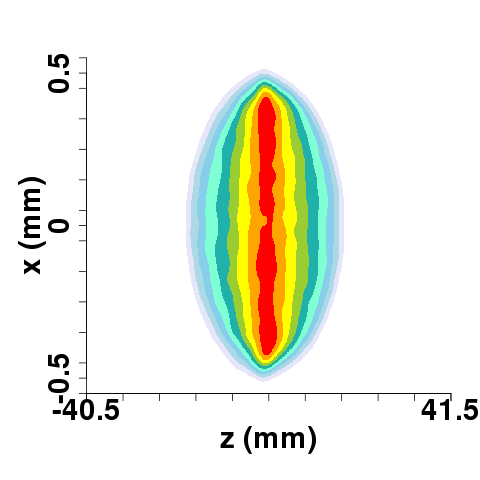
\includegraphics[width=0.2\textwidth]{figures/xz_full_dist_1e5x10_10MV-per-m.png}}&
    \subfloat[full x-y]{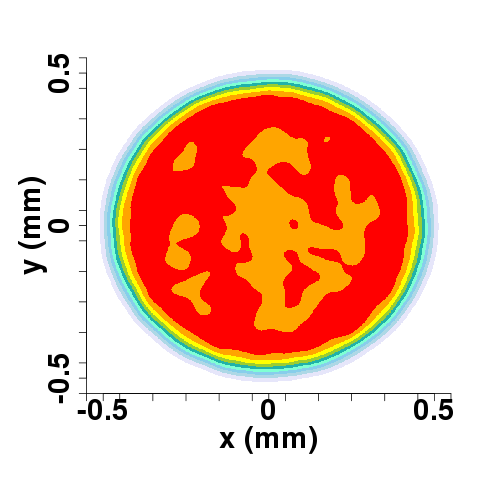
\includegraphics[width=0.2\textwidth]{figures/xy_full_dist_1e5x10_10MV-per-m.png}}&
   \\[-3mm]
    \subfloat[sliced z-x]{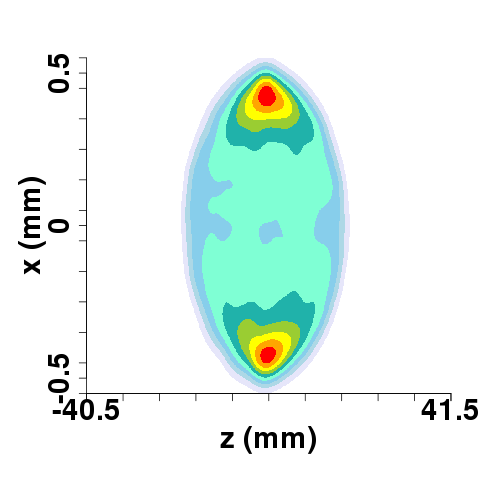
\includegraphics[width=0.2\textwidth]{figures/xz_slice_dist_1e5x10_10MV-per-m.png}}&
    \subfloat[sliced x-y]{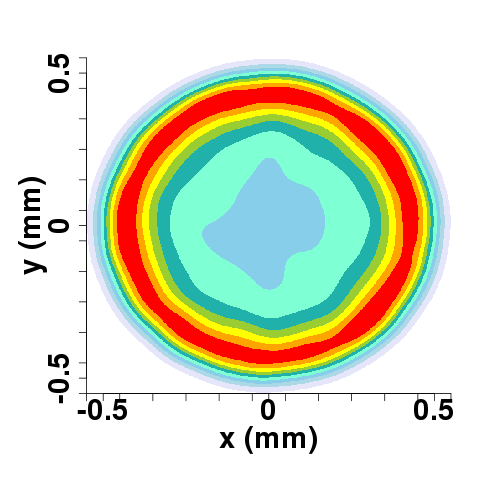
\includegraphics[width=0.2\textwidth]{figures/xy_slice_dist_1e5x10_10MV-per-m.png}}&
     \multirow{2}{*}[8cm]{\subfloat[sliced radiationl evolution]{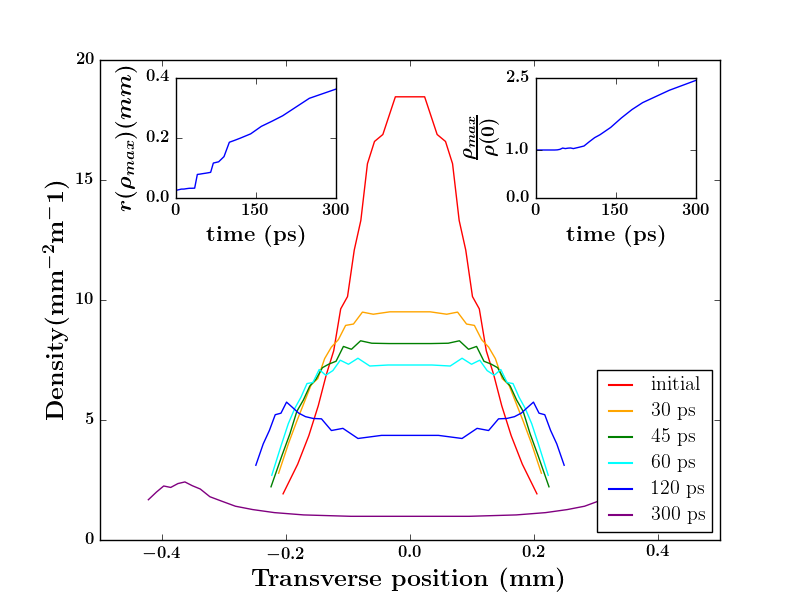
\includegraphics[width=0.6\textwidth]{figures/experiment_radial_density_up_to_300ps.png}}}\\
  \end{tabular}
\caption{\label{fig:distribution substructure} (a-d.) Two dimensional projections of $1 \times 10^6$ electron positions
simulated with the N-particle code, COSY, for approximately 300 ps after injection with a Gaussian 
($\sigma_r = 100 ~\mu m$) transverse profile into
a cavity with an electric field of 10 MV/m.  Colors are
from white to red representing linear ranges.  Other
simulations (not shown) have confirmed the presence of the ring-like density after nanoseconds.
(a.)  and (b.) are projections
of the full distribution to the x-z and x-y planes, respectively.  (c.) and (d.) are x-z and x-y
projections, respectively, of just the portion of the
distribution within 20\% of the standard deviation of the median value of y and z, respectively.  Notice
the ring-like substructure that is evident in the ``slices", (c.) and (d.) but is absent from the full distribution
projections, (a.) and (b.). (e.) N-particle radial-distribution obtained near the longitudinal median plane of the bunch at various times.
Density is calculated by binning 1000 macroparticles and assigning the resulting density to the average radial position.  The 
initial distribution is approximately Gaussian, and the square-like nature of the plot results from the discreteness of the bins.   
The sub-graph in the upper left corner shows 
the position of max density as a function of time, which is non-zero at initial time due to binning resulting in a non-zero minimum radial position. 
The sub-graph in the upper right shows the ratio of the
max density to the density at the minimum r value.  Notice, the ``phase transition" in the 45-80 ps range where the 
location of the non-zero, non-stochastic peak first appears well away from the origin. 
}
\end{figure*} 

On the other hand, an 
attractive theoretical observation relevant to a number
of fields is 
that an ellipsoidal cloud of cool, uniformly distributed
charged particles has a linear electric field within the ellipsoid which results in maintenance of the 
uniform charge density as the cloud spreads \cite{Grech:2011_coulomb_explosion}.    
In the UEM community, such a uniform distribution is a prerequisite 
in employing techniques such as emittance compensation \cite{Rosenzweig:2006_emittance_compensation}.
To create such uniform charge distributions, it has long been proposed that the formation of a uniform ellipsoid may be generated through
proper control of the transverse profile 
of a short charged-particle bunch emitted from a source into vacuum\cite{Luiten:2004_uniform_ellipsoidal}, 
and experimental results have shown that  
an electron cloud emitted from a photocathode and accelerated into the highly-relativistic regime has a shadow that is characteristics of 
such a uniform distribution\cite{Musucemi:2008_generate_uniform_ellipsoid}.  Contrary to
expectations from the free expansion work but consistent with the longitudinal analyses, this shadow
lacks any indication of a peripheral region of high-density as expected from free-expansion studies.
However, recent work has indicated that a substantial high density region may indeed form in
the transverse direction\cite{Williams:2017_transverse_emittance}, and N-particle simulation results, as
demonstrated in Fig. (\ref{fig:distribution substructure}), demonstrate a substantial
ring-like region of high density circumscribing the median of the bunch.
  
Here we demonstrate the formation of a ring-like high-density region
within both N-particle and particle in cell (PIC)
simulations of electron bunches with initial transverse Gaussian profile
and offer an explanation on why this phenomena has not been noted previously
within the UEM literature.  
We then utilize a Poisson fluid approach to derive analytic predictions 
for the dynamics of high charge density particle systems under one-dimensional, 
cylindrical, and spherical geometries
that should be relevant to a large number of physical communities, and we derive conditions 
for the emergence of density peaks distinct from any initial density maximum.
We show that peak formation has a strong dependence on 
dimension, with one dimensional systems having strict conditions on parameters for bunching whereas higher
dimensional systems have strict conditions on parameters to prevent bunching.   Additional PIC and
N-particle simulations are 
used to validate the analytical predictions for peak emergence
derived from the analytical charged-particle dynamics.  

One reason that this phenomenon has not been seen previously 
is apparent in Fig. (\ref{fig:distribution substructure}).  Previous studies, including our own work,
have looked at the projection of the distribution to the x-z plane\cite{Luiten:2004_uniform_ellipsoidal,Musucemi:2008_generate_uniform_ellipsoid,Portman:2014_image_charge,Morrison:2013_measurement,Li:2008_quasiellipsoidal}. 
Fig. (\ref{fig:distribution substructure})
shows that by projecting the distribution in this manner with the ability to only discern
density fluctuations at about the 10\% level results in the density substructure primarily along the bunch
median is lost; however,
by restricting the projection to only electrons near the median of the bunch, a restriction that can only
be done computationally presently, results in evidence of a transverse ring-like density substructure near the median longitudinal 
position.  Therefore, the full density projection obscures this signal suggesting possible substructure information is lost 
by this analytic strategy at typical density-detection resolutions.  

\begin{figure*}
  \centering
   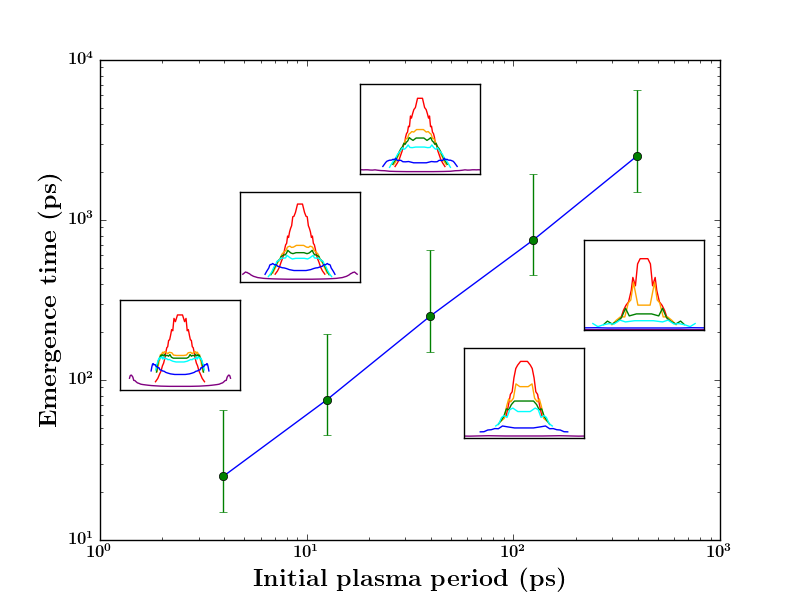
\includegraphics[width=0.75\textwidth]{figures/emergence_time.png}
\caption{\label{fig:emergence time vs plasma period} Qualitative observation of emergence of the ring-like density pulse 
as a function of initial plasma period, $\tau_p = \sqrt{\frac{m \epsilon_0}{q^2 n}}$, with $n$ representing the number density,
of the bunch as predicted by N-particle simulations.  Sub-graphs show the normalized-density evolution within 5x the initial transverse standard 
deviation of the bunch
taken at time points of roughly 0 (red), 2.5 (yellow), 3.75 (green), 5 (blue), 10 (cyan), and 25 (purple) times the plasma period
and are directly above or below their corresponding point. 
Normalized density are calculated by 
binning a number of macroparticles and assigning the resulting density to the average radial position as was also done in
Fig (\ref{fig:distribution substructure}e).  The 
initial distribution is Gaussian, and the square-like nature of the sub-plots results from the discreteness of the bins.   
Notice that the density pulse is more prominent in the higher-dose distributions but is evident in all simulations emerging
somewhere in the $2.5 \tau_p$ to $10 \tau_p$ range indicated on the main plot by error bars despite the presence
of more stochastic effects in the lower doses.  Low dosage (corresponding to the three larger
plasma period times) plots fail to capture the full width of
the bunch at 25 $\tau_p$ due to spreading beyond $\pm 0.5$ m resulting from the initial velocity spread and the long density pulse
emergence time; however, we have kept the scale to demonstrate the main features of the density pulse evolution. Due to the 
large error bars of the density pulse emergence time resulting from the qualitative nature of the observation, 
we do not provide the equation of the line here.  
}
\end{figure*} 

A second reason that this phenomenon has not been seen previously 
is apparent in Fig. (\ref{fig:emergence time vs plasma period}) which presents a qualitative description of
when to expect the emergence of the ring-like substructure.  Specifically, 
most analytic work has been conducted using $\le~10\text{k}$ electrons with a
transverse standard deviation of 100 $\mu$m, and this structure is
not apparent for at least 500 ps.  Moreover, even when using the slicing 
analytic strategy, this structure is barely discernible from stochastic noise.  Also, as can be seen
in Fig. (\ref{fig:emergence time vs plasma period}), the pulse emergence time is essentially
a constant factor times the plasma period.  We derive
the corresponding factor explicitly for cylindrical and spherical symmetries later in this manuscript.

%Table

Due to the appearance of this ring-like phenomenon in both 
N-particle and PIC simulations, we conclude that applying a mean-field like reasoning 
applied to the transverse expansion of the bunch should be able to
capture the gross dynamics.  Distilling this reasoning, a distribution that is originally more dense 
toward the center, then particles toward the center should experience more radial force resulting in an inverse velocity chirp
that results in ring-like build-up of electrons.  However, it is not immediately apparent why such dynamics are almost
entirely absent in the 
longitudinal direction as found by numerous studies \cite{Luiten:2004_uniform_ellipsoidal,Siwick:2002_mean_field,Reed:2006_short_pulse_theory}; therefore, we develop a theory to describe this understanding in one, two, and three dimensions
where analytic progress is possible due to the unique properties of the Coulomb interaction in 
special symmetric geometries. 

Consider 
the non-relativistic spreading of a electron bunch in a one dimensional model, which is a good approximation 
to the longitudinal spreading of a pancake-shaped electron cloud generated at a photocathode. 
In one dimensional models, the charge density only depends on 
one co-ordinate, which we take to be the $z-axis$.  For the sake of readability,
denote $z = z(t)$ and $z_0 = z(0)$ and denote the charge distribution at all times to
be $Q_\text{tot} \rho(z,t)$ with $\rho(z,t)$ 
a unitless, probability-like density and  
$Q_\text{tot}$  the total charge in the bunch.  Further, abbreviate $\rho(z_0,0)$ as $\rho_0$.
In one dimensional models, the amount of distribution to either side of the particle 
determines the field at the particle resulting in a monotonic electric field, and in the absence of any particle crossover, this field, and hence the resulting
particle acceleration, $a(z,t)$ is independent of time providing
$a(z,t) = a(z_0,0)$ abbreviated as $a_0$ and thus suggesting that
the details of the density evolution are captured by the relation between
$z$ and $z_0$.
However, due to the constant nature of $a_0$, this 
relation is the elementary constant acceleration kinematic equation
\begin{equation}\label{eq:non-relativistic position}
  z = z_0 + v_0 t + {1\over 2} a_0 t^2
\end{equation}
where $v_0$ is the initial velocity of the charged particle at $z_0$.  In general,
both $v_0$ and $a_0$ are functions of the initial position, $z_0$, and the special case of $v_0 = 0$ everywhere, which we will call the cold-case,
is commonly assumed in the literature.  Notice, that particle crossover should never occur in the cold case resulting in this description being valid
for 1D cold case dynamics for all time. 

Since particles may neither be created nor destroyed in our model, we have
\begin{equation}
\rho(z,t) dz = \rho_0 dz_0
\end{equation}
so that in the non-relativistic case derived above,
\begin{align}
  \rho(z,t) &=  \rho_0 \left({dz\over dz_0}\right)^{-1} ={ \rho_0} \over  {1 + v_0' t +\frac{1}{2} a_0' t^2} \label{eq:1D density evolution}
\end{align}
where $v_0' = \frac{dv_0}{dz_0}$ 
and $a_0' =  \frac{da_0}{dz_0}$.
Consider a freely expanding initial charge distribution that is symmetric and initially centered at  
$z=0$ in the non-relativistic limit.   The charge distribution evolves under the influence of the internal space charge 
forces leading to
\begin{equation}\label{eq:delta acceleration}
  a_0 = \frac{q Q_\text{tot}}{2 m \epsilon_0}  {\delta \sigma},
\end{equation}
where $q$ is the charge of the particle, $m$ is its mass, and 
\begin{equation}
  \delta \sigma = \int_{-z_0}^{z_0} \rho_0(z) dz,
\end{equation}
Notice via the Fundamental Theorem of Calculus
that the derivative of the acceleration with respect to the initial position is
directly proportional to the initial distribution
\begin{align}\label{eq:first order acceleration}
  a_0' &= \frac{q Q_\text{tot}}{2 m \epsilon_0}  \frac{d{\delta \sigma}}{dz_0}\nonumber\\
          &= \frac{q Q_\text{tot}}{m \epsilon_0}\rho_0
\end{align}
where the symmetric nature of $\rho_0$ was used to eliminate the factor of $2$.
Plugging Eq. (\ref{eq:first order acceleration}) into Eq. (\ref{eq:1D density evolution}), we get
\begin{align}
  \rho(z,t) &=  { \rho_0 \over  1 + v_0' t +  \frac{q Q_\text{tot}}{2 m \epsilon_0} \rho_0t^2}\label{eq:1D density evolution subbed}\\
  \frac{d}{dz} \rho(z,t) &= \frac{ \rho_0'\left( 1  + v_0' t\right) - \rho_0v_0''t }{\left(1 + v_0' t +  \frac{q Q_\text{tot}}{2 m \epsilon_0} \rho_0t^2\right)^3}\label{eq:1D rho derivative} 
\end{align}
where $\rho_0' = \frac{d\rho_0}{dz_0}$ and $v_0'' = \frac{d^2v_0}{dz_0^2}$. A 
detailed derivation of the second expression is done in the Supplemental.  
For the cold-case, 
Eq. (\ref{eq:1D density evolution subbed}) 
reduces to  density evolution
derived by Reed\cite{Reed:2006_short_pulse_theory}.  Also, in the cold-case,
Eq. (\ref{eq:1D rho derivative}) simplifies into a proportionality
between the initial slope of the distribution and the slope of the distribution at
any later time.  
Therefore, a charge distribution that is initially at rest and unimodal, i.e only
a single initial location has non-zero density with $\rho_0' = 0$,  
never develops 
a dynamically generated second maximum.
This explains why we should not expect to see a density ridge in the longitudinal direction
while the 1D model is applicable in the cold-pancake regime.
The extension of this description to asymmetric functions is straightforward, as is the inclusion of an 
image field at the photocathode.  However, inclusion of these effects does not change
Eq. (\ref{eq:1D density evolution subbed}), Eq. (\ref{eq:1D rho derivative}), nor the conclusions
we have drawn from them.  The non-cold case will be discussed elsewhere.

The constant acceleration approximation and absence 
of particle crossovers is not valid in the cylindrical and 
spherical geometries, nevertheless analytic results are still possible prior to 
particle crossover in the non-relativistic regime.   Consider a non-relativistic evolving distribution 
$Q_\text{tot} \rho(r,t)$, where $\rho(r,t)$ is again taken to be the unitless
particle distribution and $Q_\text{tot}$ is again the total charge in the bunch.    In a system with cylindrical symmetry,
the mean field equation of motion for a charge at $r \equiv r(t)$ is given by,
\begin{equation}\label{eq:2D second derivative}
  \frac{d \vec{p}_\text{2D}}{dt} = { q Q_\text{tot} \lambda (r,t)\over 2 \pi \epsilon_0 r}\hat{r} 
\end{equation}
where $\lambda(r,t)$ is the linear charge inside radius $r$ calculated by
$\lambda(r,t) = \int_0^{r} 2\pi \tilde{r} \rho(\tilde{r},t) d\tilde{r}$ again
normalized so that $\lambda(r,t) \le 1$.
Analogously in a system with spherical symmetry,
the equation of motion for an electron at position $r$ is given by
\begin{equation}\label{eq:3D second derivative}
  \frac{d \vec{p}_\text{3D}}{dt} = { q Q_\text{tot} Q(r,t)\over4\pi \epsilon_0 r^2}\hat{r} 
\end{equation}
where $Q(r,t) = \int_0^{r} 4\pi \tilde{r}^2 \rho(\tilde{r},t) d\tilde{r}$ again normalized so
$Q(r,t) \le 1$.  Notice, $r$ in Eq. (\ref{eq:2D second derivative}) denotes the cylindrical radius while
$r$ in Eq.  (\ref{eq:3D second derivative}) represents the spherical radius
, and the ambiguity will be maintained
throughout the text.  In both situations, before
any crossover occurs, the charge integrals 
are constant.  That is, we may write
$\lambda(r,t) = \lambda(r_0,0) \equiv \lambda_0$
and $Q(r,t) = Q(r_0,0) \equiv Q_0$ for a particle starting at $r_0 \equiv r(0)$.
$Q_\text{tot} \lambda_0$ and $Q_\text{tot} Q_0$ can be 
interpreted as the charged contained in the appropriate Gaussian surface,
and if we track the particle that starts at $r_0$, these contained charges should remain constant
before any crossover occurs.
It is convenient to also define the average particle density to be
$\bar{\rho}_0 = \frac{\lambda_0}{\pi r_0^2 }$ in the 2D case and 
 $\bar{\rho}_0 = \frac{Q_0}{\frac{4\pi r_0^3}{3} }$ in the 3D case.  Notice that
 this average particle densities are a function solely of $r_0$, and
 we will use later in the text.
Eq. (\ref{eq:2D second derivative}) and 
Eq. (\ref{eq:3D second derivative}) may now be rewritten as 
\begin{align}
  \frac{d p_{r,\text{2D}}}{dt} &= { q Q_\text{tot} \lambda_0\over 2 \pi \epsilon_0 r}\label{eq:2D equation of motion}\\ 
  \frac{d p_{r,\text{3D}}}{dt} &= { q Q_\text{tot} Q_0\over 4 \pi \epsilon_0 r^2}\label{eq:3D equation of motion}
\end{align}
for the period of time before particle crossover and where all time dependence in the force is accounted for by the
$r$ term in the denominator.

 Since Eq. (\ref{eq:2D equation of motion}) and Eq. (\ref{eq:3D equation of motion}) 
 represents the force on the particle in the cylindrical and spherical contexts, respectively, 
 we can integrate over the particle's 
 trajectory to calculate the change in the particle's energy. 
 Integrating from $r_0, 0$ to $r, t$ gives
\begin{align}
  E_\text{2D}(r,t) - E(r_0,0) &= \frac{q Q_\text{tot} \lambda_0}{2 \pi \epsilon_0} ln\left(\frac{r}{r_0}\right)\label{eq:2D energy}\\
  E_\text{3D}(r,t) - E(r_0,0) &= \frac{q Q_\text{tot} Q_0}{4 \pi \epsilon_0} \left(\frac{1}{r_0} - \frac{1}{r}\right)\label{eq:3D energy}
\end{align}
where the term on the right side of the equality can be interpreted as  the change in the potential energy within the self-field
of the bunch.  

These expressions are fully relativistic, and in the non-relativistic limit, we can derive the position-time relation for the particle.
The details of this derivation have been placed in the on-line Supplement, and the resulting expressions in the cold-case are presented here
\begin{align}
  t_\text{2D} &= \frac{\bar{\tau}_{p,0}}{\pi} \frac{r}{r_0} F\left(\sqrt{ln\left(\frac{r}{r_0}\right)}\right)\label{eq:2D time}\\
  t_\text{3D} &= \sqrt{\frac{3}{2}}\frac{\bar{\tau}_{p,0}}{2\pi} \left( \tanh^{-1} \left( \sqrt{1 -  \frac{r_0}{r}} \right) + \frac{r}{r_0}\sqrt{1 -  \frac{r_0}{r}}\right)\label{eq:3D time}
\end{align}
where $F(\cdot)$ represents the Dawson function and $\bar{\tau}_{p,0}$ represents the plasma period 
determined from the initial conditions
by $\bar{\tau}_{p,0} = 2\pi \sqrt{\frac{m\epsilon_0}{q Q_\text{tot} \bar{\rho}_0}}$ indicating that the
appropriate time scale is essentially the plasma period as determined qualitatively in Fig. (\ref{fig:emergence time vs plasma period}).
The expression for time in the spherically symmetric case, $t_\text{3D}$, has been derived previously \cite{Last:1997_analytic_coulomb_explosion}.
Furthermore, the time-position relation detailed in these equations depends solely on the amount of charge 
nearer to the origin than the point in question, i.e. $Q_\text{tot} \bar{\rho}_0$, consistent with 
Gauss's law and not on the details of the distribution.  Notice, however,
that each initial position can have a different time constant, and that it is the relationship between the 
time-position relationships of different locations where the details of the distribution become important and may cause
neighboring particles to have interesting relative dynamics.  

To understand these dynamics we generalize Eq. (\ref{eq:1D density evolution}), 
\begin{align}
  \rho(r,t) = \rho_0 \left( \left(\frac{r}{r_0}\right)^{d-1} {\frac{dr}{dr_0}}_\text{d}\right)^{-1}\label{eq:density evolution general}
\end{align}
where d is the dimensionality of the problem, i.e. 1, 2 or 3 in this text.
The factor in the denominator, ${\frac{dr}{dr_0}}_\text{d}$, may be 
determined implicitly from the time-position relations above, as we've done this in general in the Supplement
We again present the expressions in the cold case for $d=2$ and $d=3$
\begin{align}
  \frac{d r}{dr_0}_\text{d} &= \frac{r}{r_0} \left(1 + \frac{d}{2} \left(\frac{\rho_0}{\bar{\rho}_0} - 1\right) f_\text{d}\left(\frac{r}{r_0}\right)\right)\label{eq:dr over dr_0 no v_0}
\end{align}
where $ f_\text{2}\left(\frac{r}{r_0}\right) = 2  \sqrt{\ln\left(\frac{r}{r_0}\right)}F\left(\sqrt{\ln\left(\frac{r}{r_0}\right)}\right)$ and
$f_\text{3}\left(\frac{r}{r_0}\right) = \frac{r_0}{r} \sqrt{1 - \frac{r_0}{r}} \tanh^{-1}(\sqrt{1 - \frac{r_0}{r}}) + 1 - \frac{r_0}{r}$.  For further analysis, call
$D_\text{d} = D_\text{d}(r_0) = \frac{d}{2} \left(\frac{\rho_0}{\bar{\rho}_0} - 1\right)$ the divergence from uniform function in 2 and 3 dimensions.
These $D$ functions are solely functions of the initial conditions and are positive at locations where the local density is larger than the average density, negative when the density
is smaller than the average density, and identically zero when the average density is identical to the local density. 
Specifically, for a uniform distribution with an infinitely sharp cutoff in either the cylindrical or spherical case, the 
corresponding $D$ function is zero at every location where the original density is defined.  Thus, the uniform density evolution
in Eq. (\ref{eq:density evolution general})
reduces to the generally recognized [citations] $\rho(r,t) \pi r^2=  \rho_0 \pi r_0^2$ in the cylindrical case and $\rho(r,t) \frac{4}{3} \pi r^3=  \rho_0 \frac{4}{3} \pi r_0^3$ in
the spherical case.  However, Eq. (\ref{eq:dr over dr_0 no v_0})
is general for any distribution before particle crossover, not just the uniform distribution.

\begin{figure}
  \centering
  \subfloat[$f_\text{2}\left(\frac{r(t)}{r(0)}\right)$]{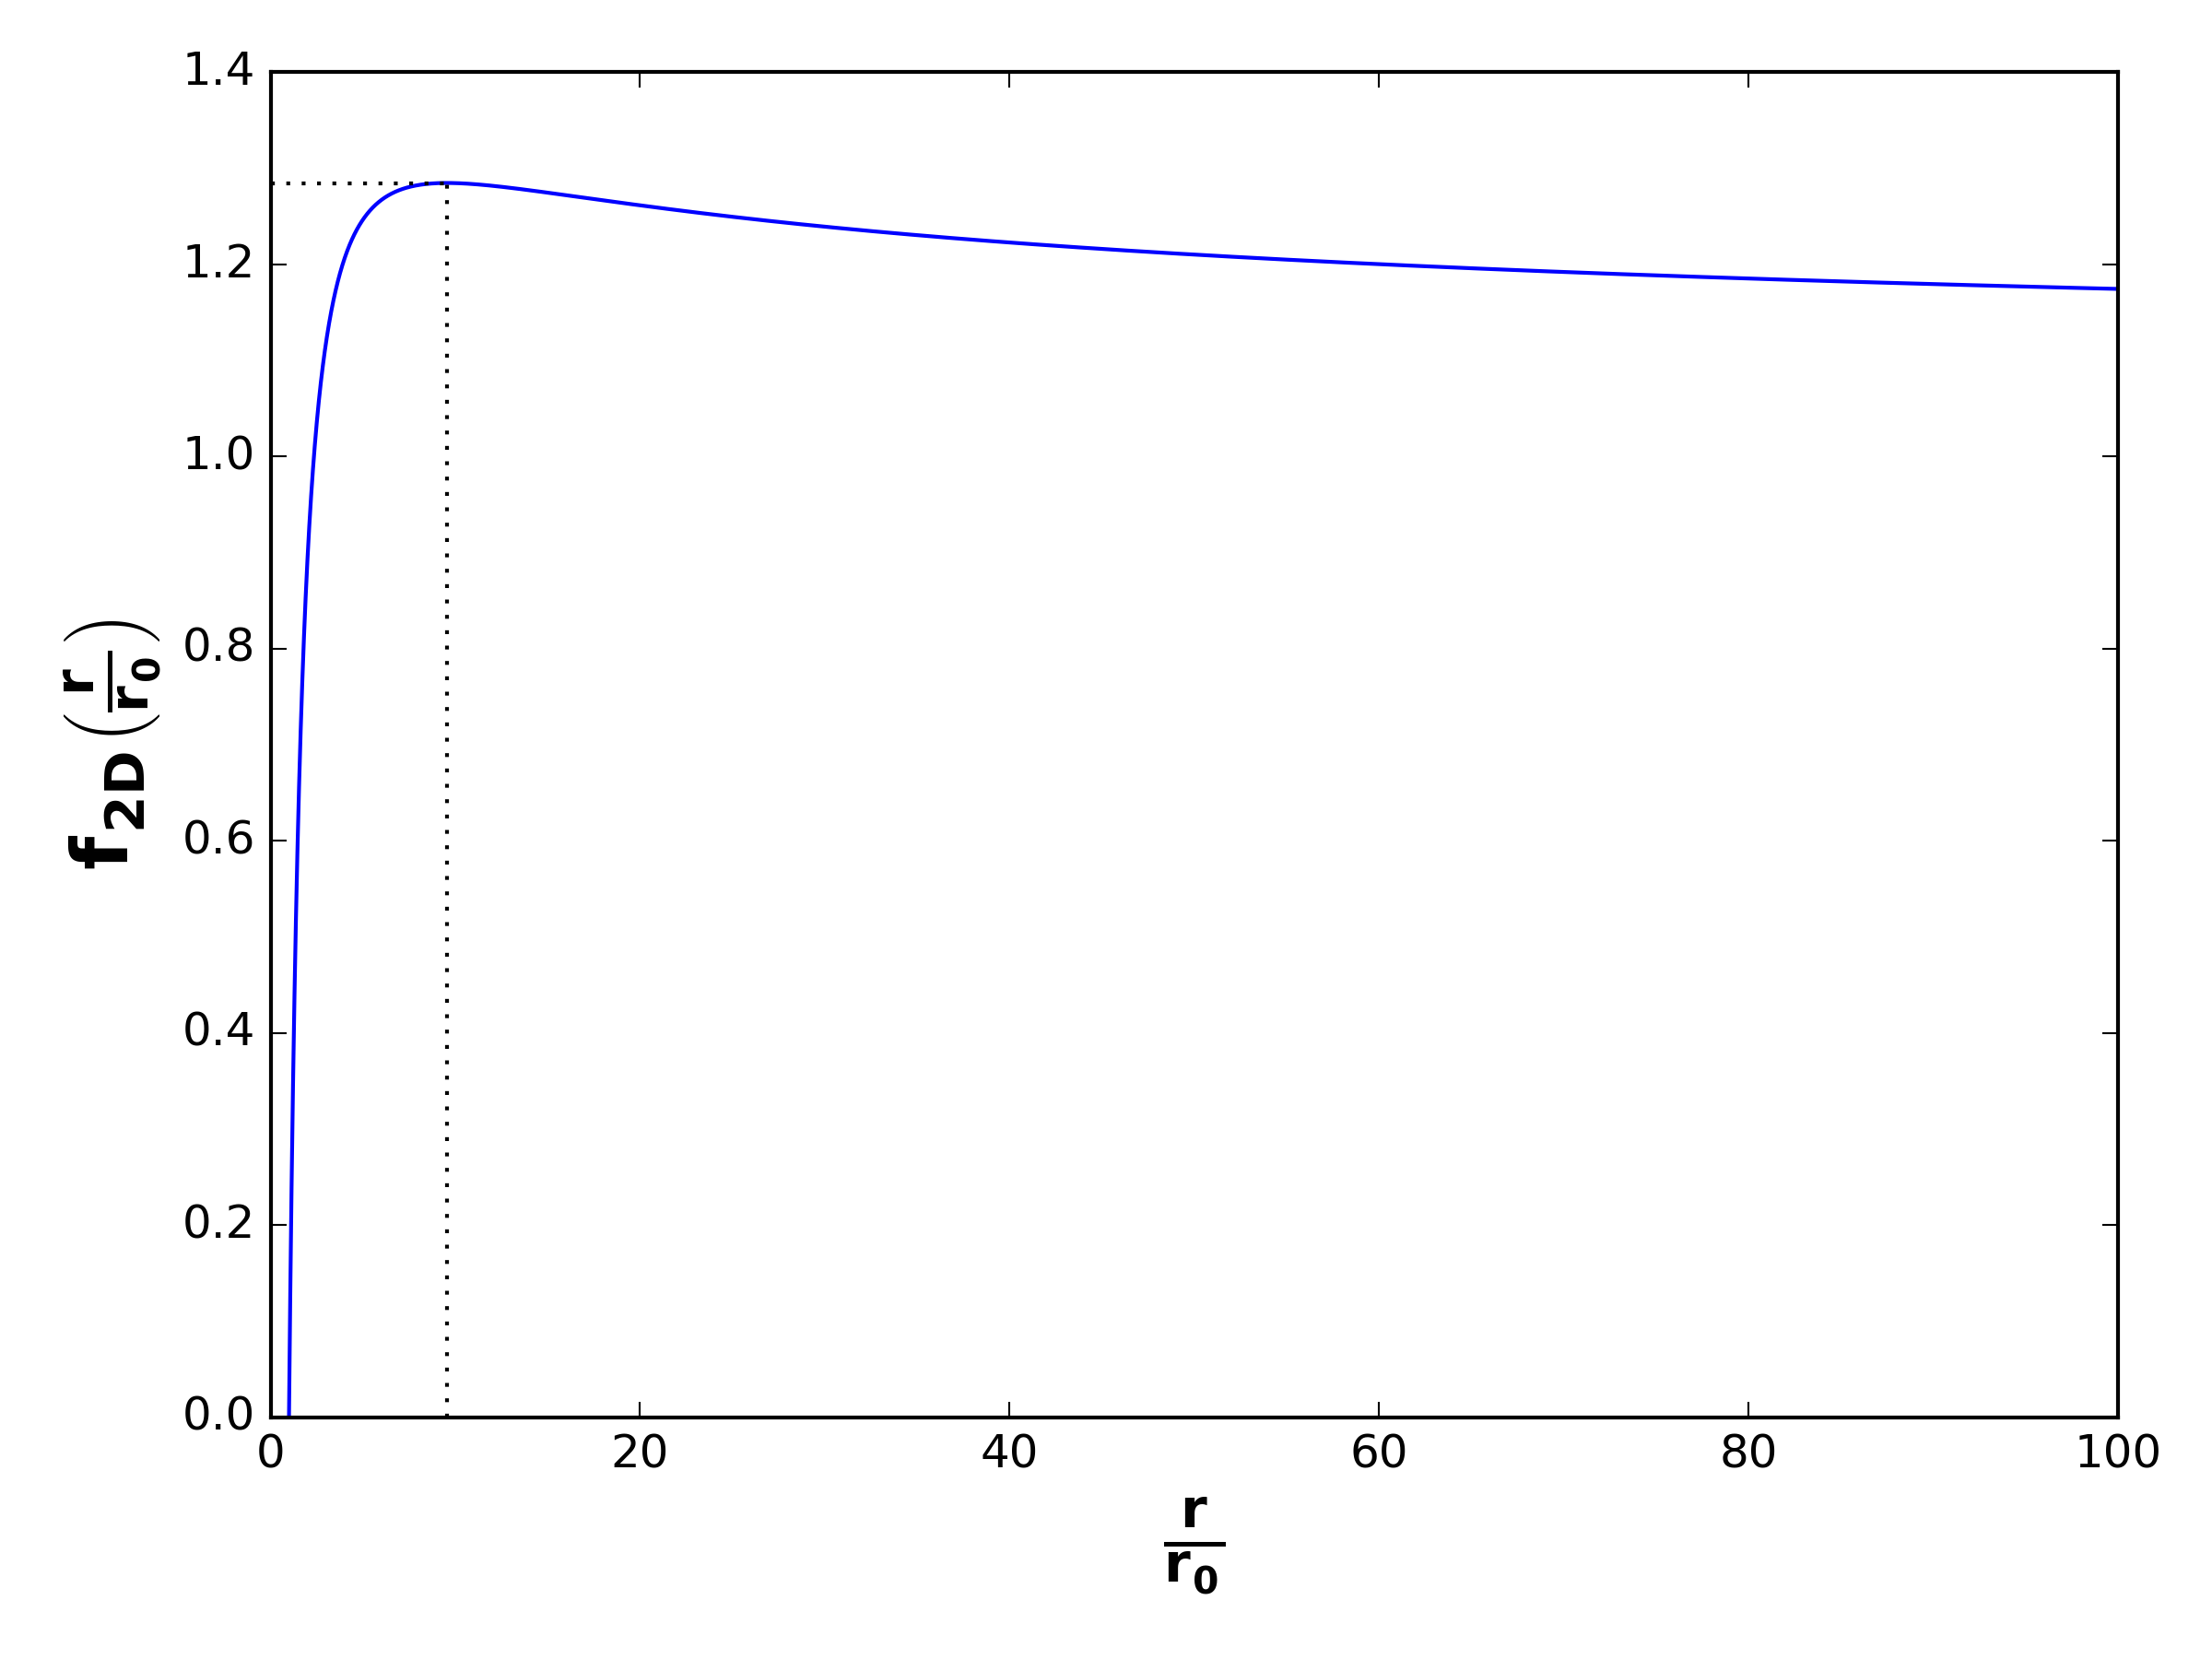
\includegraphics[width=0.24\textwidth]{figures/logarithmic_scaling_coefficient_function.png}}
  \subfloat[$f_\text{3}\left(\frac{r(t)}{r(0)}\right)$]{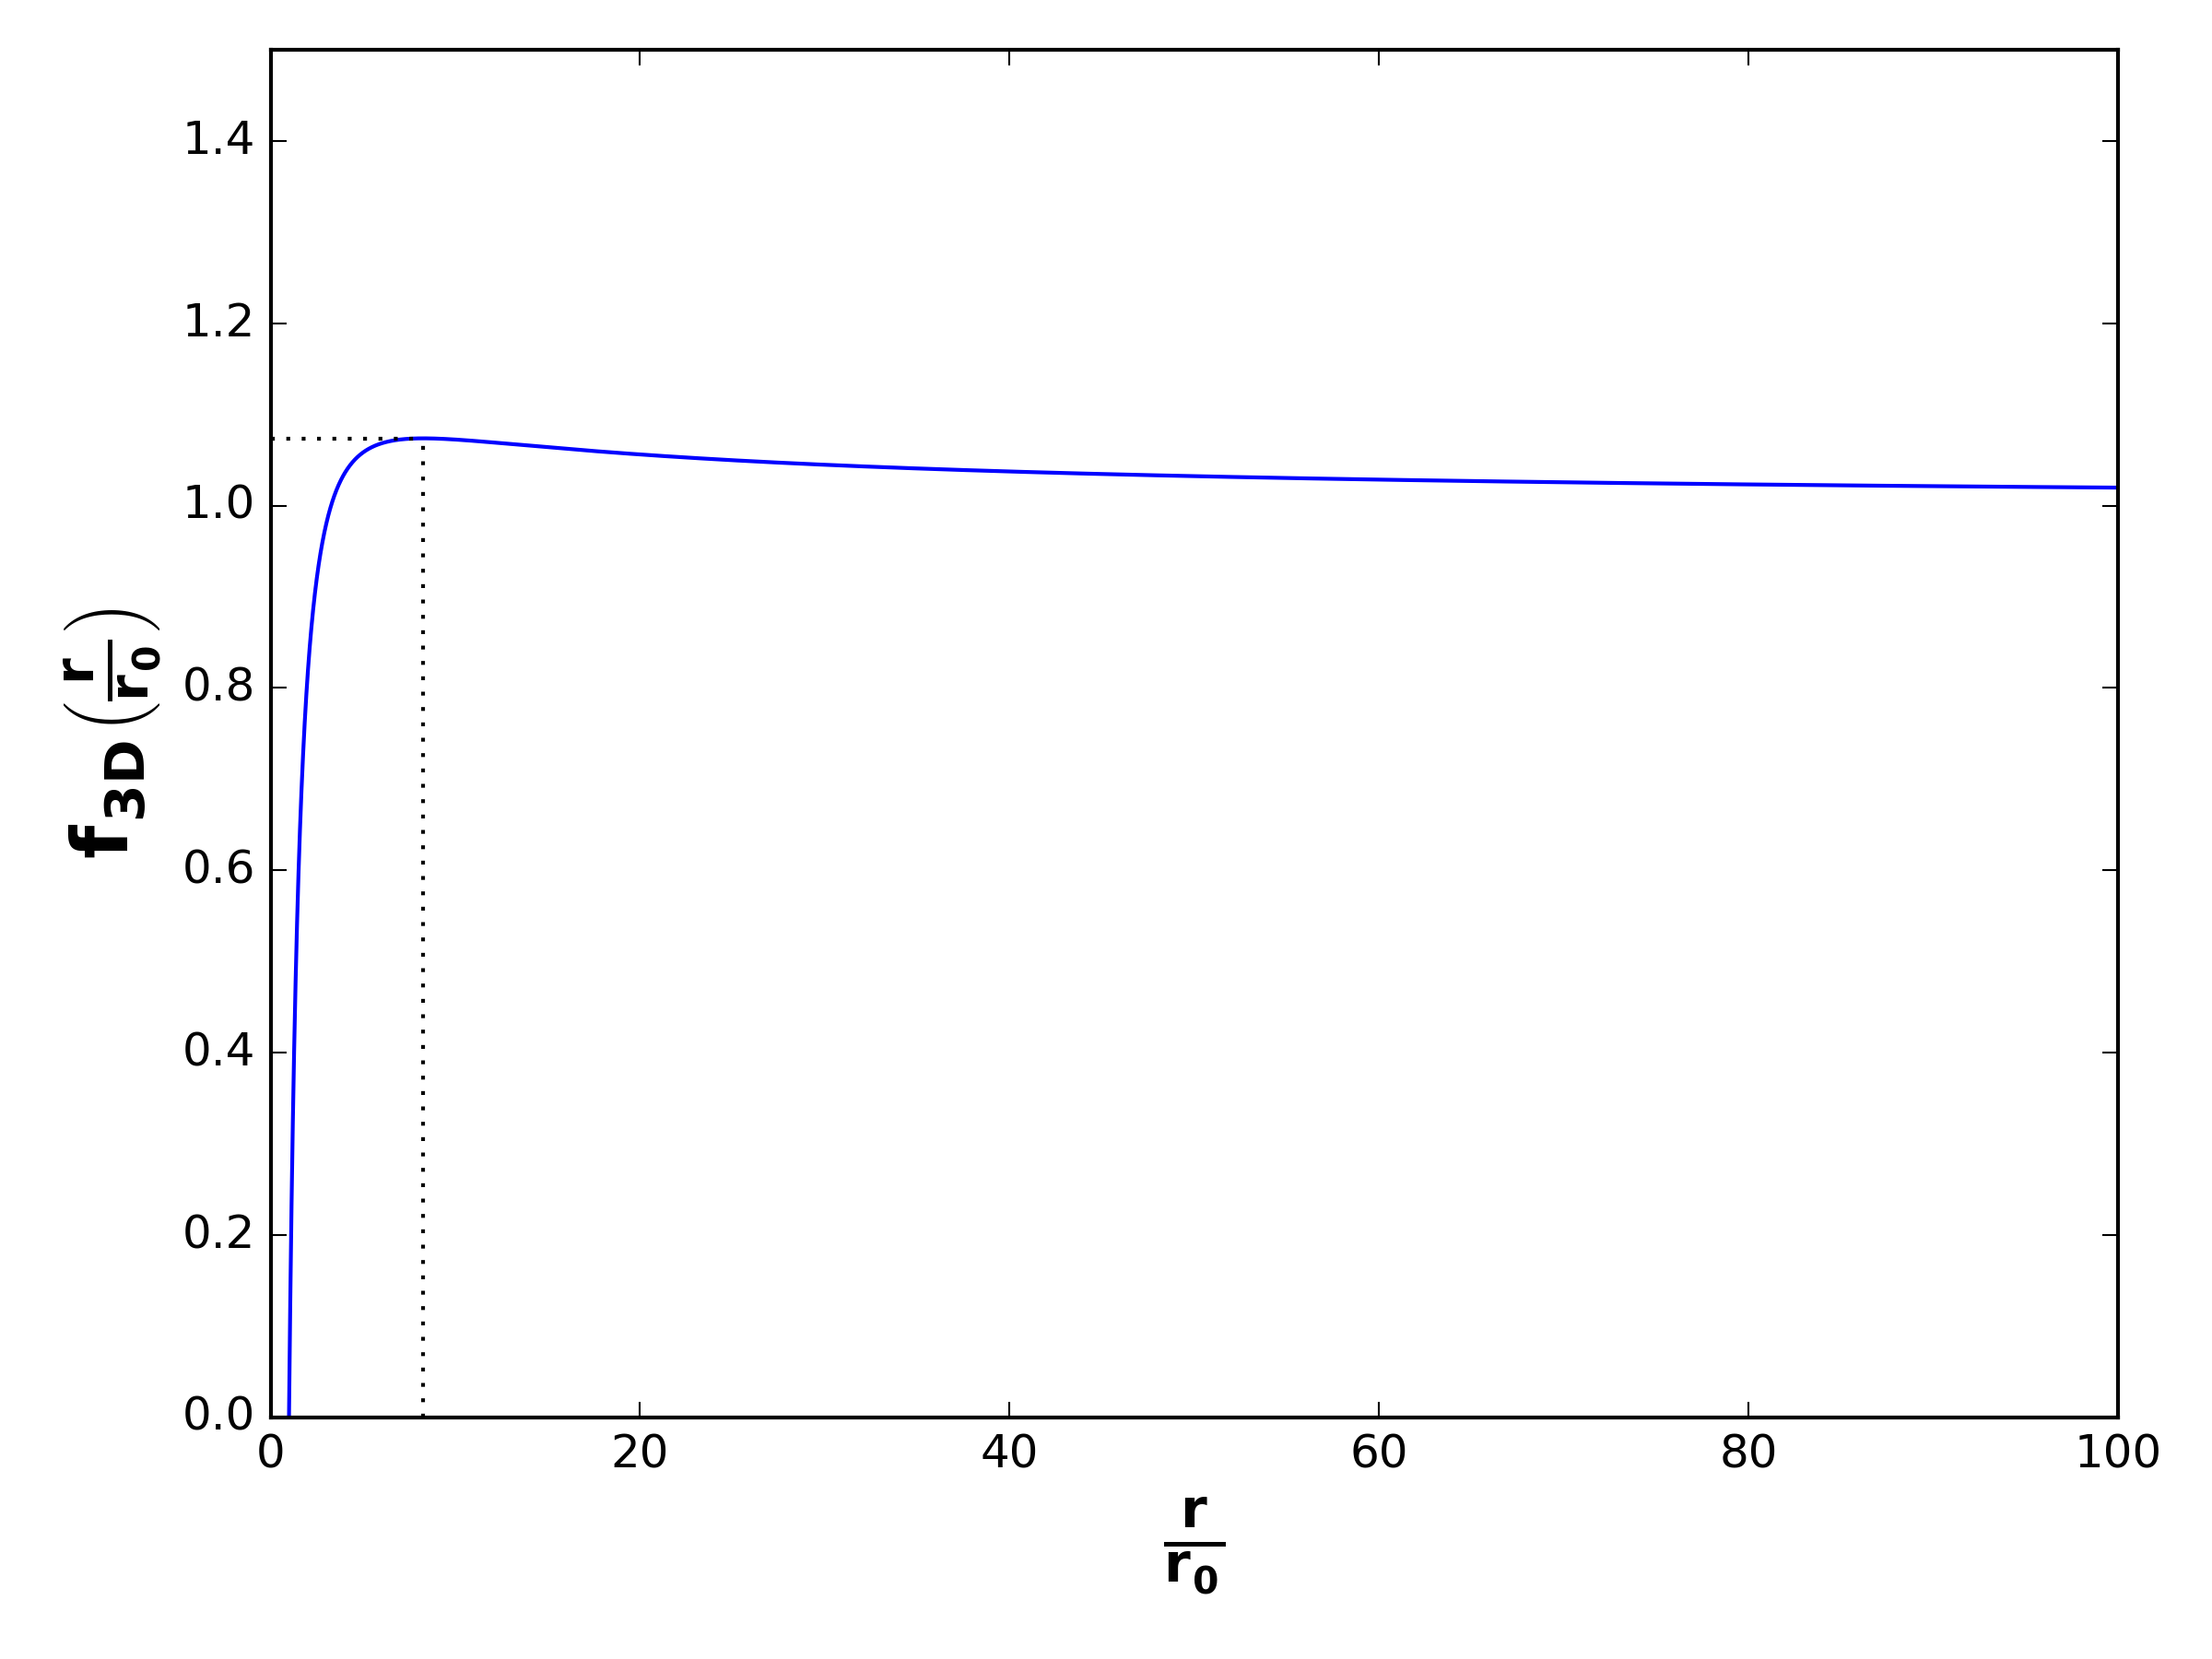
\includegraphics[width=0.24\textwidth]{figures/inverse_scaling_coefficient_function.png}}\\
  \subfloat[$D_\text{2}(r(0))$ classification]{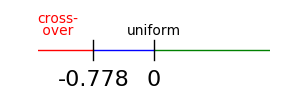
\includegraphics[width=0.24\textwidth]{figures/d_line_2.png}}
  \subfloat[$D_\text{3}(r(0))$ classification]{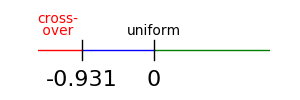
\includegraphics[width=0.24\textwidth]{figures/d_line.png}}
\caption{\label{fig:classifying D} (a-b.) Plot of the $f_\text{2D}$ and $f_\text{3D}$ functions against $\frac{r}{r_0}$.  
Since particles are always expanding in our model, $\frac{r}{r_0} \ge 1$ and goes to infinity for infinite time.  Notice that
both functions have similar character with a maximum in the $8-10 ~ r_0$ range eventually approach1 from above.  Dashed lines
indicate the location of the functions' maximum.  These functions allow
us to classify the distribution by the initial value of $D_\text{dD}(r_0) = \frac{d}{2} \left(\frac{\rho_0(r_0)}{\bar{\rho}_0(r_0)} - 1\right)$
as is done in (c-d.).  Specifically, regions experiencing crossover (local contraction), in red, the uniform distribution, when 
$D_\text{dD}(r_0) = 0$, and regions experiencing more or less expansion than the uniform distribution, in green and blue, respectively
are marked in the figures.}
\end{figure} 

Again, analogous to the one dimensional case, particle crossover occurs when $\frac{d r}{d r_0}_\text{d} = 0$.  
For a particle starting at position $r_0$ and having a divergence from uniform function $D_\text{d}(r_0)$, crossover occurs when the particle is at 
a position, $r$, that satisfies $f_\text{dD}(r,r_0) = -1/D_d(r_0)$.  Since every particle expands in this model, every particle will have a time for which it will assume every value of the function $f(r,r_0)$.  The character of the two and three dimensional $f$'s are similar as can be seen in Fig (\ref{fig:classifying D}) where
the value of the function is plotted against $\frac{r_0}{r}$.
Specifically, both functions increase to a maximum and then asymptote towards 1 from above.  
This means that all density positions eventually experience uniform-like scaling since $\lim_{r \to \infty} f_{dD}(r,r_0) = 1$
 results in Eq. (\ref{eq:density evolution general}) simplifying to $\rho \pi r^2 =  \rho_0 \frac{\pi r_0^2}{1 + D_\text{dD}(r_0)}$ and 
$\rho \frac{4}{3} \pi r^3=  \rho_0 \frac{\frac{4}{3} \pi r_0^3}{1 + D_\text{dD}(r_0)}$ in the cylindrical and spherical cases, respectively, for large enough $r$.
The main differences are that the cylindrical function's max is larger than the spherical function's,  $max(f_\text{2D}) \approx 1.28$ 
vs $max(f_\text{3D}) \approx 1.07$, and occurs at a larger
value of $\frac{r_0}{r}$ than the spherical function, $r \approx 9.54 r_0$ instead of $r \approx 8.27 r_0$, respectively.  The first observation means cylindrical 
symmetry is more sensitive to the distribution than spherical symmetry, whereas the second means that if crossover is going to occur for a specific particle, 
it will occur before the $r$ value for which the corresponding $f$ function is maximum (i.e. $r \approx 9.54 r_0$ or $r \approx 8.27 r_0$), 
otherwise the particle will never experience crossover.    
However, too much should not be made of this observation as once crossover has occurred 
 farther from the center of the distribution than a given point, this given point may eventually crossover the crossed over point as the crossed over point no longer can be described by 
 our model.  Nevertheless, we may obtain the earliest time of crossover before which our model is completely valid as a mean-field theory.  This can be obtained by minimizing
 the time with the crossover constraint $ {\frac{dr}{dr_0}}_\text{d} = 0$ by such methods as Lagrange multiplies, where the Lagrangian has the following form
 \begin{align}
   \mathcal{L}_\text{dD} = t_\text{dD} - \lambda\left(1 - \frac{d}{2}\left(\frac{\rho_0(r_0)}{\bar{\rho}_0(r_0)} - 1\right) f_\text{dD}(r,r_0)\right)\label{eq:Lagrangian crossover}
 \end{align}

\begin{figure*}
  \centering
  \begin{tabular}{cc}
    \subfloat[cylindrical symmetry uniform]{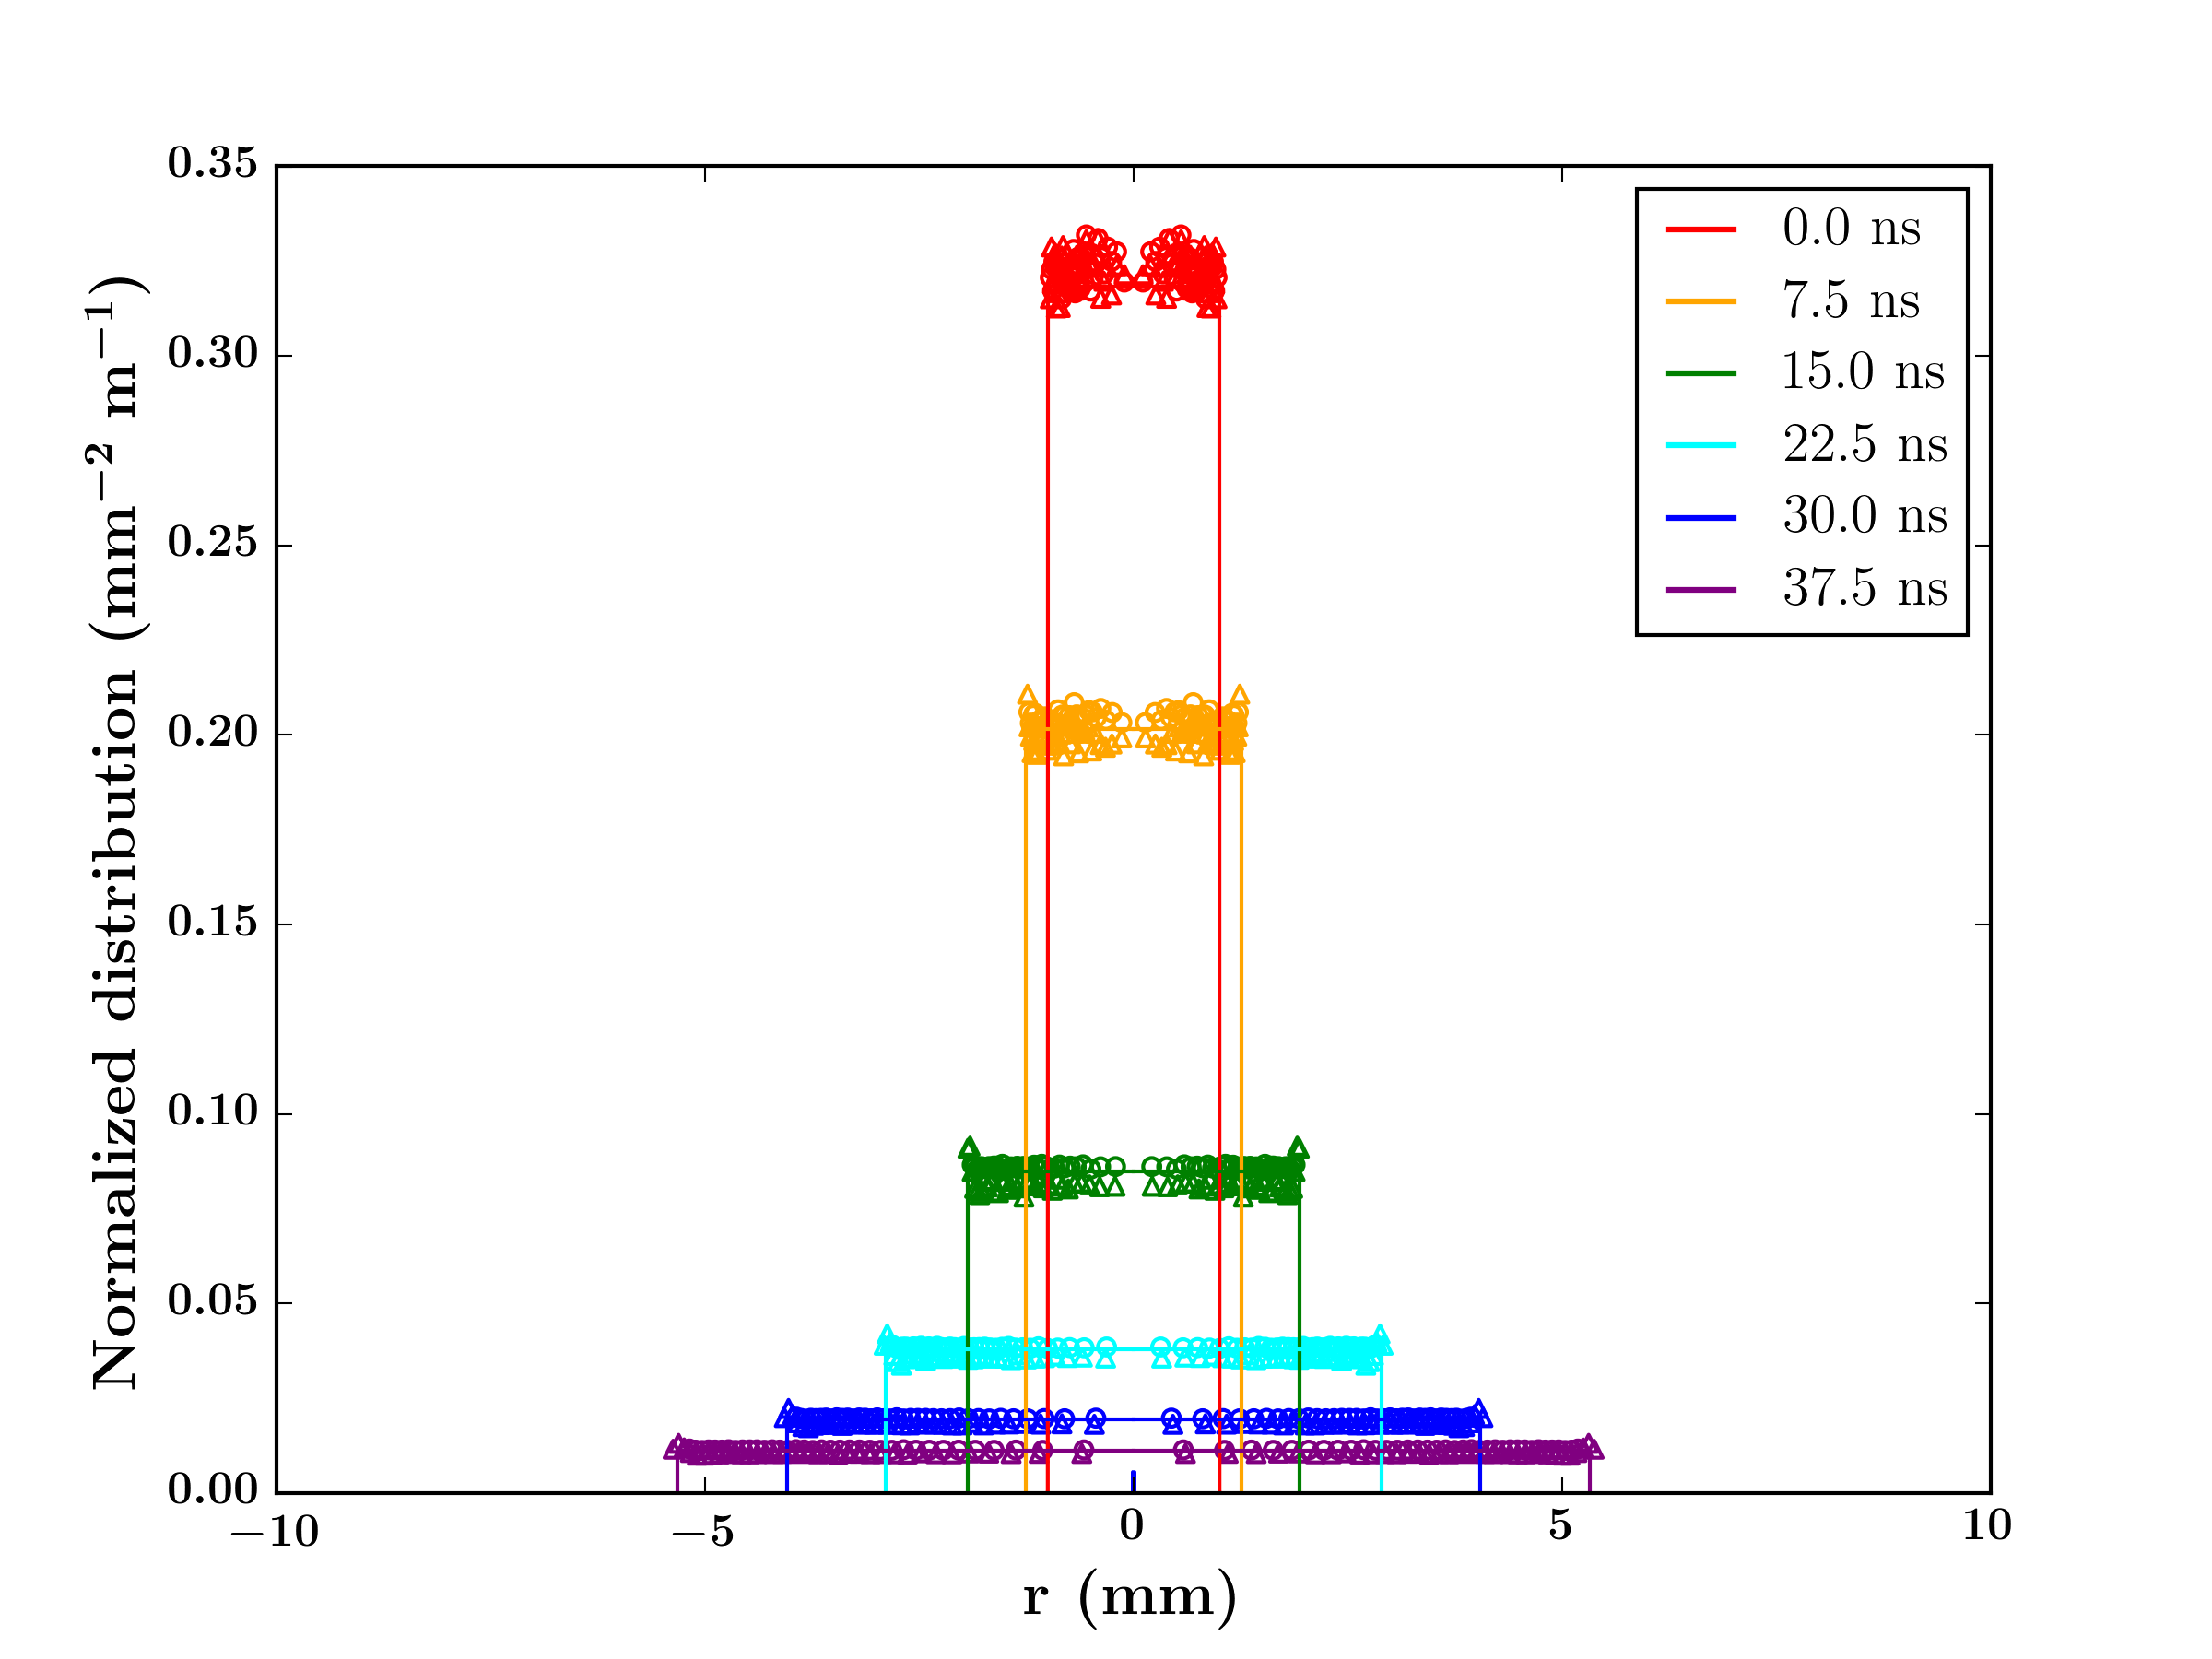
\includegraphics[width=0.5\textwidth]{figures/uniform_cylindrical_density_evolution.png}}&
    \subfloat[spherical symmetry uniform]{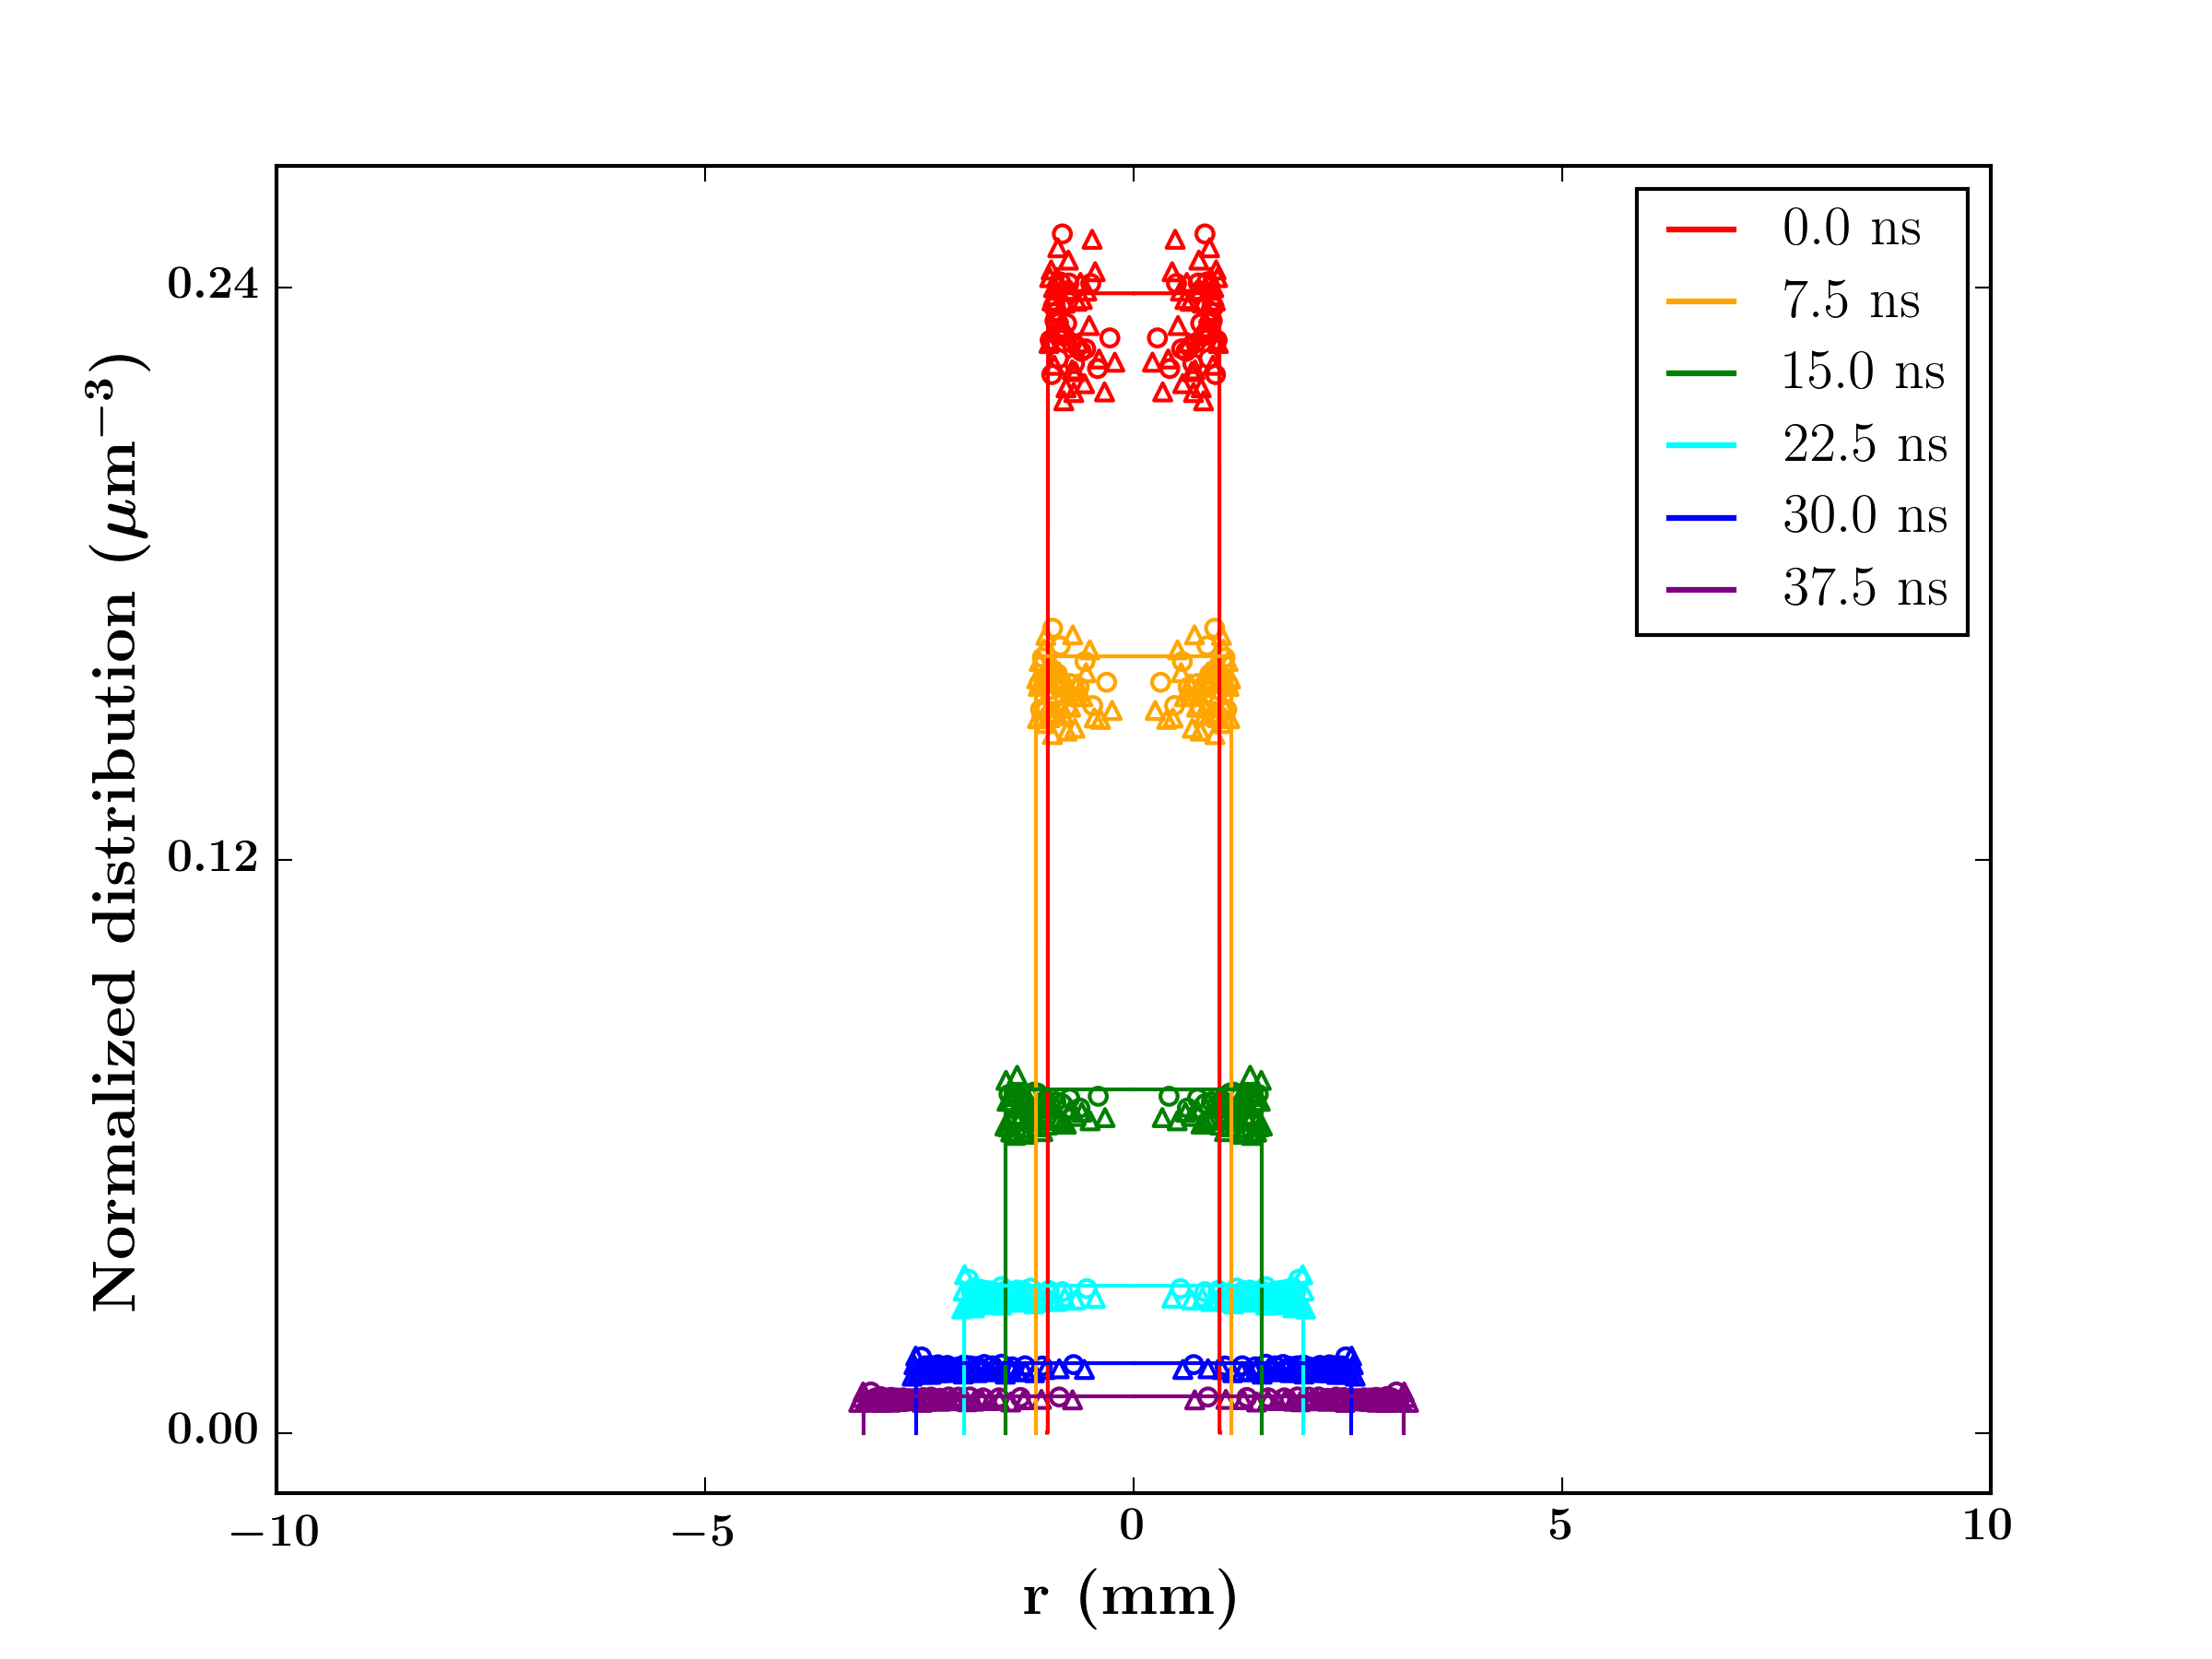
\includegraphics[width=0.5\textwidth]{figures/uniform_spherical_density_evolution.png}}
    \\
    \subfloat[cylindrical symmetry Gaussian]{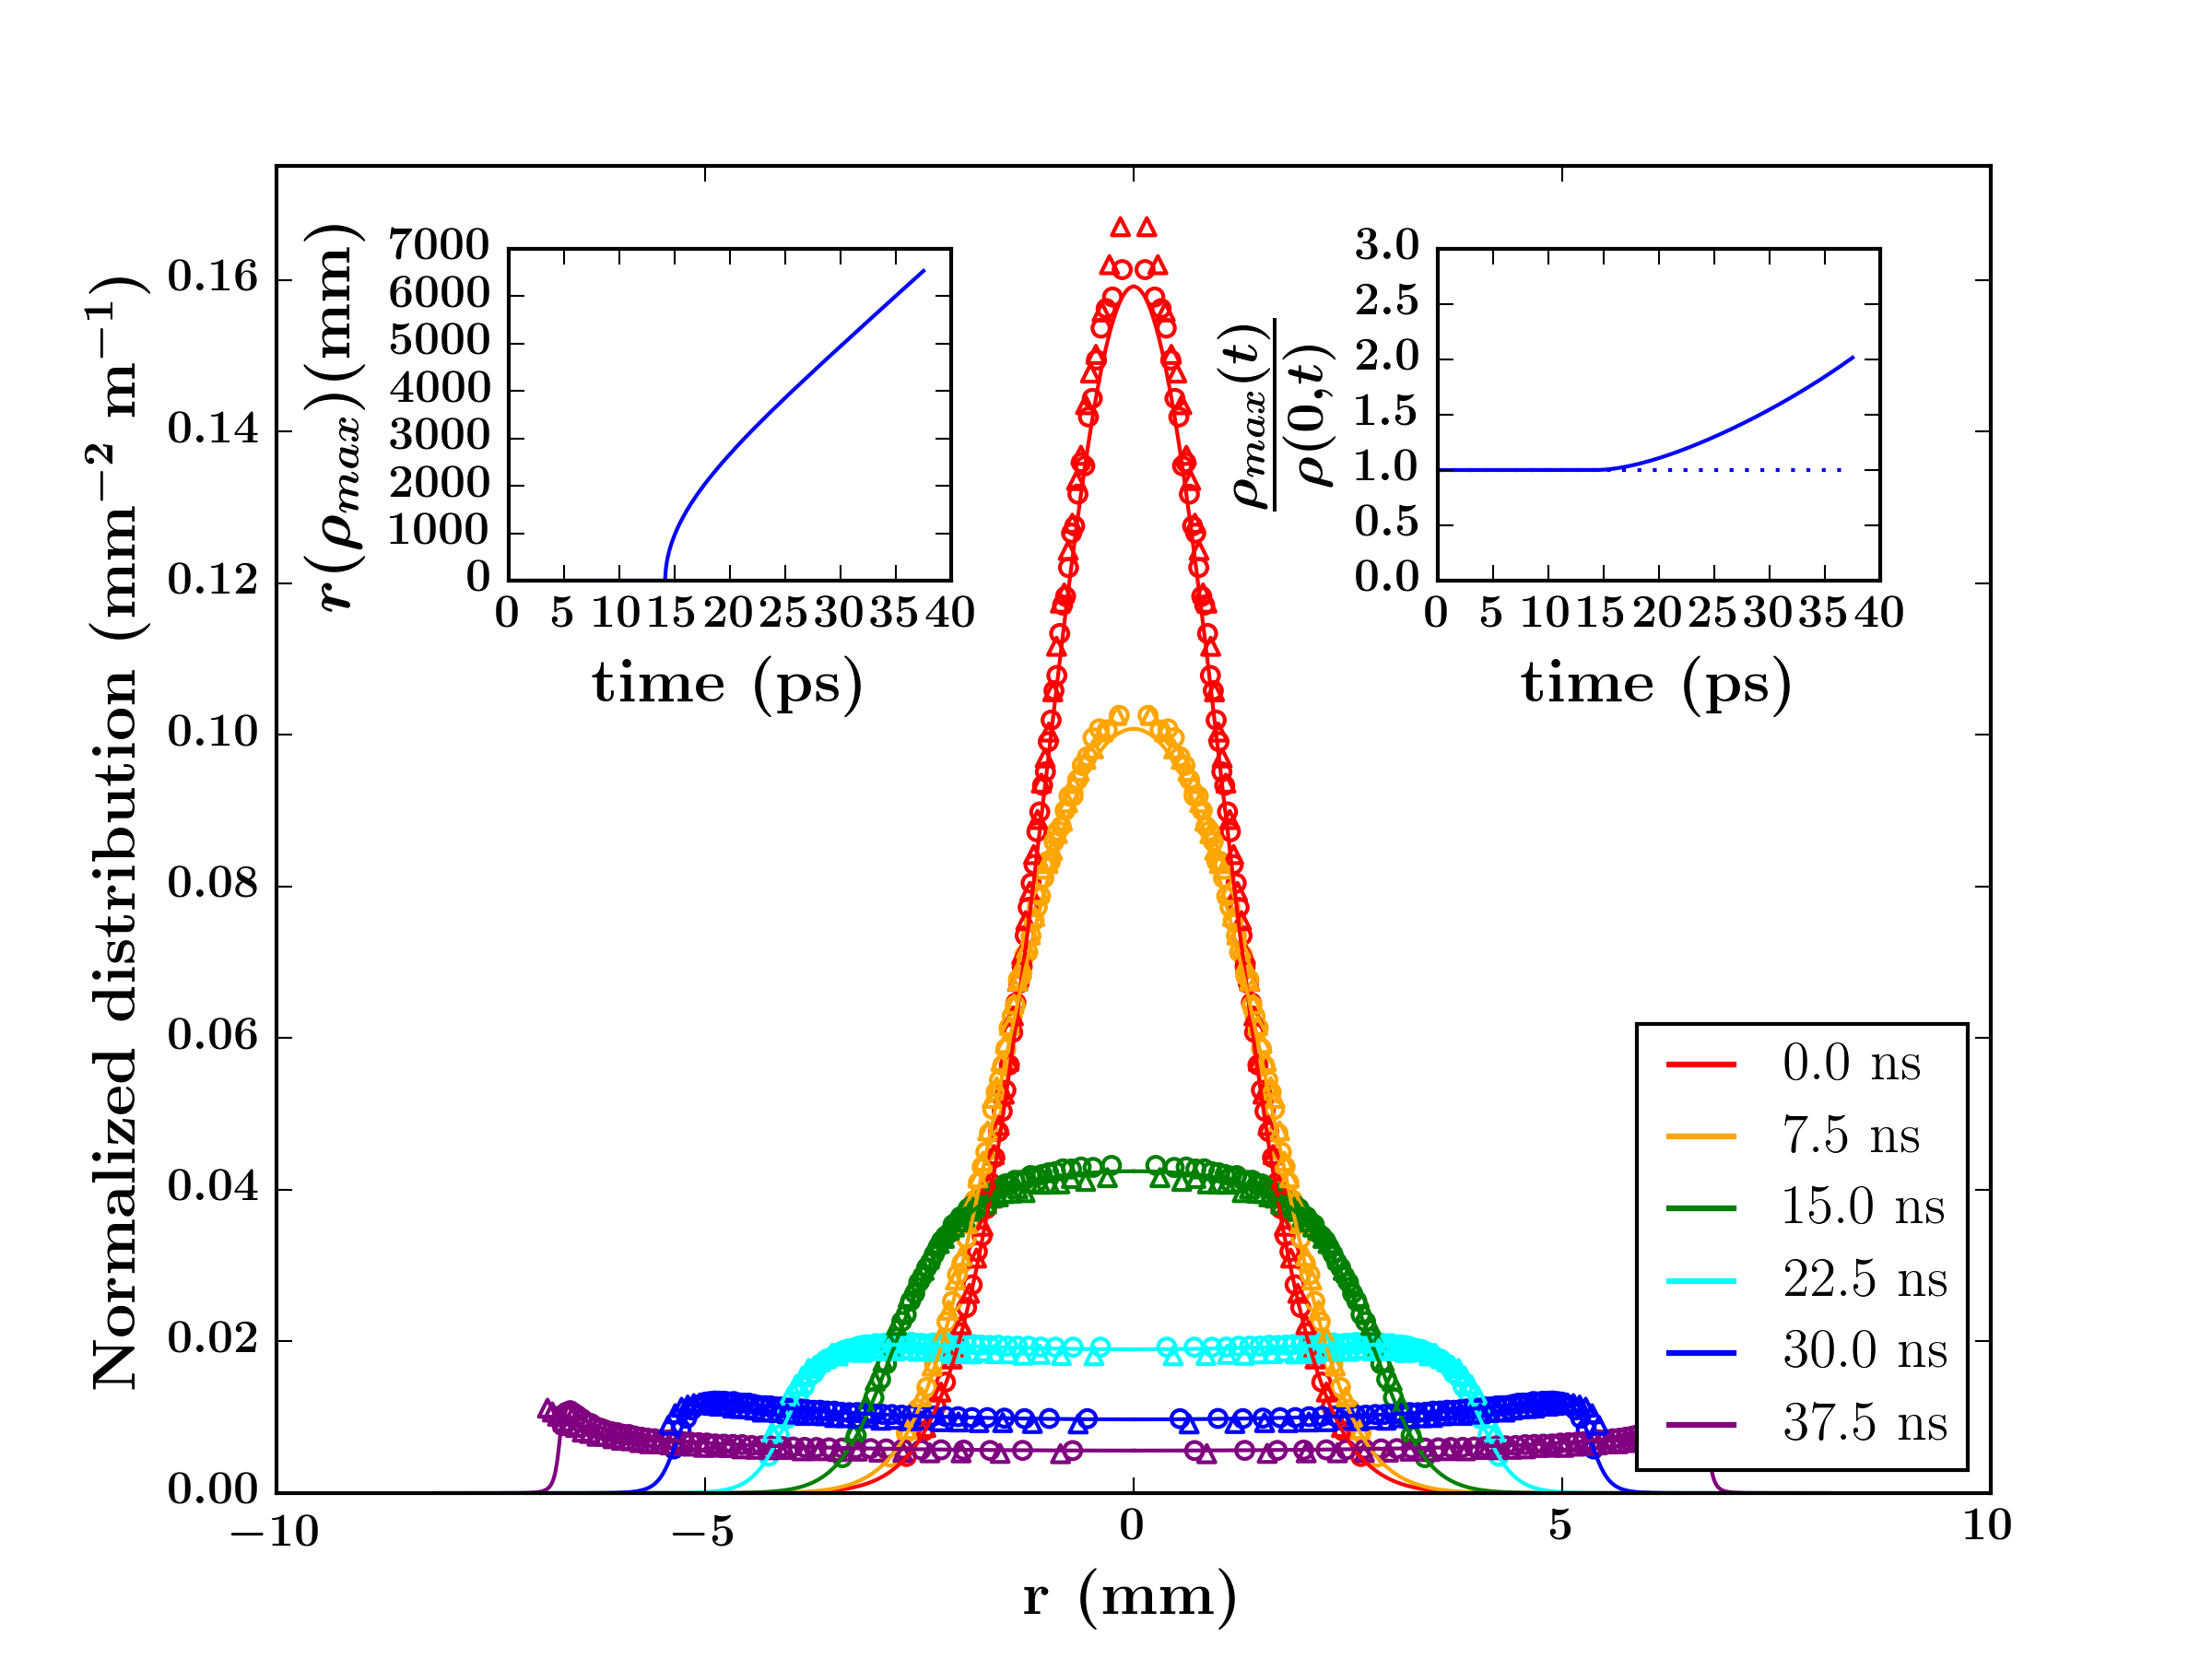
\includegraphics[width=0.5\textwidth]{figures/cylindrical_density_evolution.png}}&
    \subfloat[spherical symmetry Gaussian]{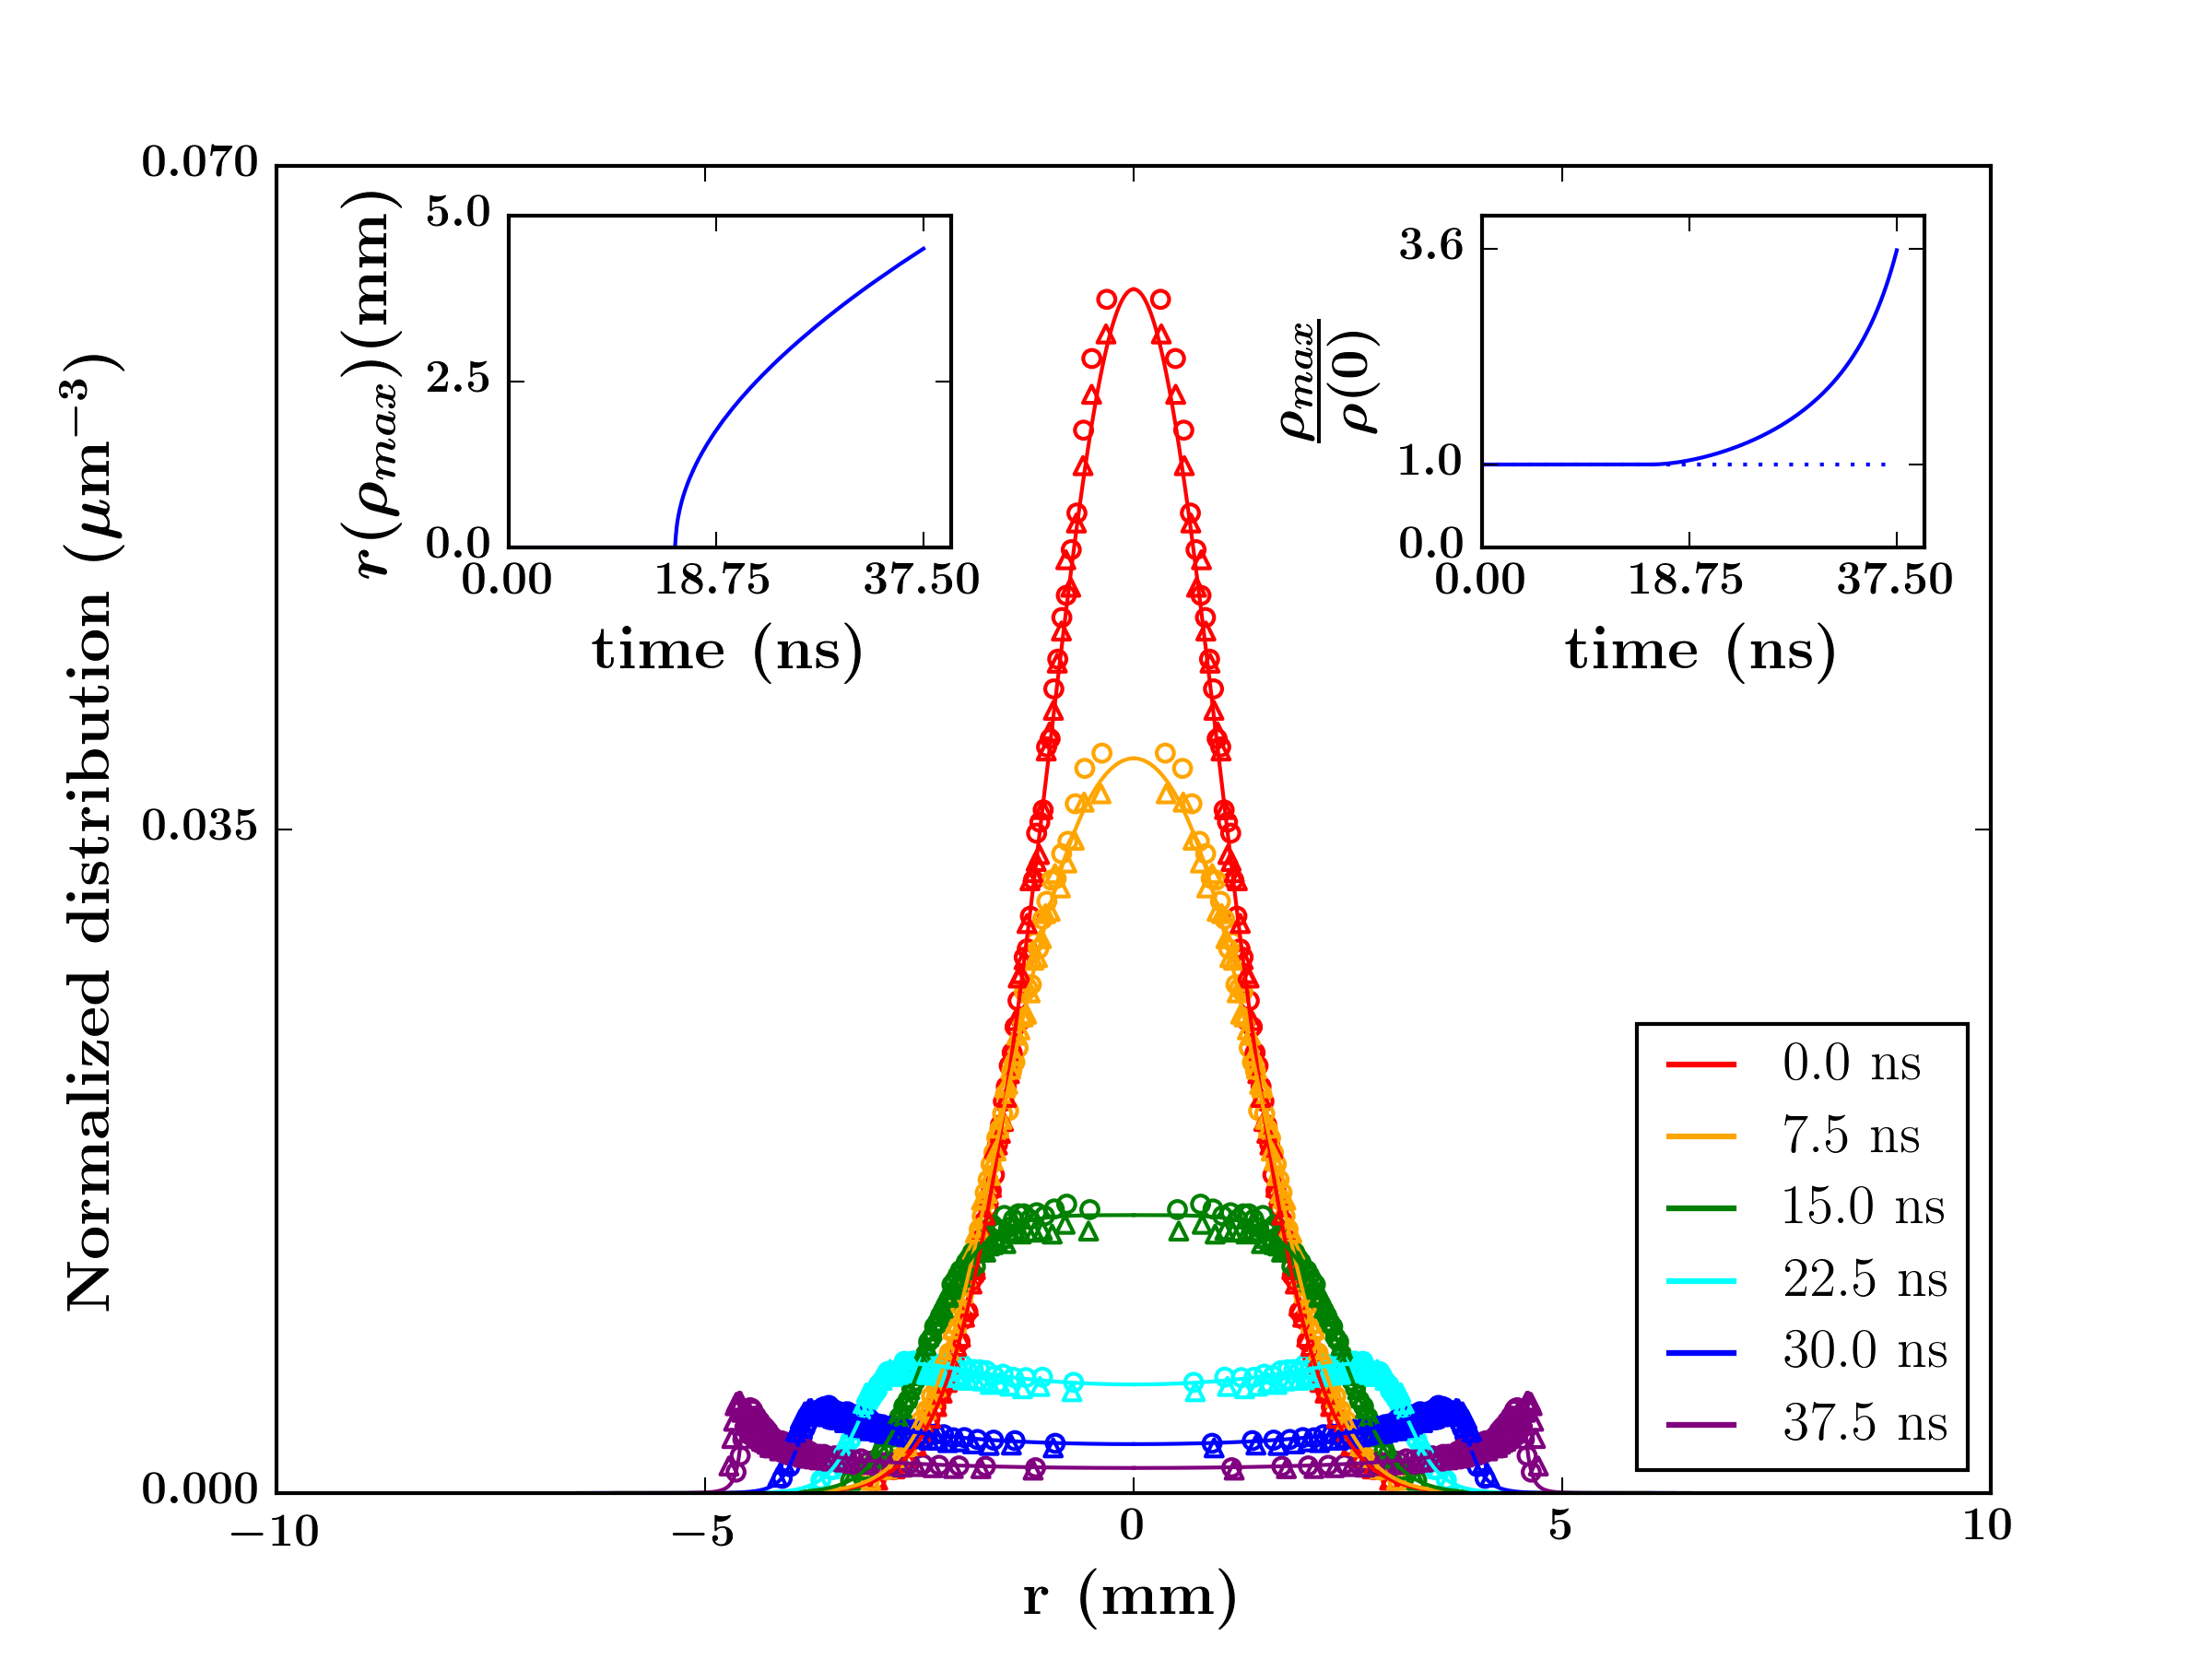
\includegraphics[width=0.5\textwidth]{figures/spherical_density_evolution_less_dense.png}}
  \end{tabular}
\caption{\label{fig:density evolution} Analytical (solid line), PIC (cirlces), and N-particle (triangles) results of the normalized density 
evolution of (a.,c.) cylindrically and (b., d.) spherically symmetric 
(a., b.) uniform and (c.,d.) Gaussian distributions with $R = \sigma_r = 1 $ mm and  $N$ of $1.875 \times 10^7$, $2 \times 10^4$, $3.75 \times 10^7$,
and $10^5$ electrons, respectively,
before any analytic crossover events.  The sub-graph
in the upper left corner of (c.,d.) shows 
the analytic position of max density as a function of time, and the sub-graph in the upper right of (c.d.) shows the analytic ratio of the
max density to the density at the minimum r value both.  The corresponding analytic ratio for the uniform distribution is shown in this sub-graph
as a dashed horizontal line at 1.   Unsurprisingly, the 
PIC results and the analytical results, both mean-field models, are in almost perfect agreement, and the N-particle results
are in surprisingly good agreement as well.
Notice that the models predict peak formation on a time-scale dependent on the initial plasma frequency similar to the peak formation seen
in the N-particle disc-like density evolution seen in Fig. (\ref{fig:distribution substructure}(e.)) and detailed in Fig. (\ref{fig:emergence time vs plasma period}).}
\end{figure*} 

To demonstrate the use of these equations, we present the evolution of the initially-at-rest cylindrically- and spherically- symmetric uniform distribution of
$1.875 \times 10^7$ and $2^4$ electrons within radii's of 1 mm (see Fig. (\ref{fig:density evolution}(a,b)).  Note, in this fairly trivial case, crossover should not 
occur and the analytic results should be valid mean-field-results for all time.  As can be seen in Fig. (\ref{fig:density evolution}(a,b)), the evolution of the uniform 
distribution in 
both PIC and N-particle simulations is captured by the analytic solution.  Specifically, the distributions simply expand while remaining uniform, 
and the analytic formulation correctly calculate the rate of this expansion.  

Less trivially is the evolution of Gaussian distributions. We simulated 
$3.75 \times 10^7$ and $10^5$ electrons for the cylindrical and spherical cases, respectively,  using $\sigma_r =1 ~$ mm.  
Solving for the minimum crossover time, 
we get approximately and 44 ns for each distribution.  Therefore, we simulate for 37.5 ns, which is well before any crossover events.  As can be seen in
Fig. (\ref{fig:density evolution}), both the cylindrically- and spherically- symmetric Gaussian distributions develop peaks similar to what is seen in our disc-like simulations,
and this ``phase-like'' transition arise on the order of approximately 20 ps.  Also, as can be seen in Fig. (\ref{fig:density evolution}), both the PIC 
and the N-particle results match the analytical
results extremely well. The primary differences between the cylindrically- and spherically- symmetric evolutions is in their rate of width expansion
and in the sharpness of the peak that forms, both of which are captured by the analytic models.  In
addition, the analysis presented here may be carried out utilizing $\rho_0(\phi,r,z) = \sigma_0(\phi,r) \delta(z - z_0)$ to model the UEM
pancake regime expansion, but this results in a slightly different interpretation of the
$D$ function than the spherical case presented above and these details will be presented elsewhere.  


\section{Conclusions}
0.  Summary of findings.
1.  Steady state Child-Langmuir current should not have this
  a.  Non-steady state bunches though... depends on profile and initial density
  b.  This possibly has wide applicability
2.  Bi-modal distributions and rms emittance
  a.  Explains Luiten's observations
  b.  Can be ameliorated at the cost of loss of electrons
3.  A deeper study of this phenomena is warranted
4.  We have not really discussed emittance, and further study on emittance is warranted.
In particular the dynamical formation of a density peak 
near the edges of the bunch, in the transverse direction, leads to opportunities 
to improve the brightness and coherence length critical to ultrafast electron 
microscopy and may be exploited in other fields.



\textit{\textbf{Acknowledgment}}
This work was supported by the Colleges of Natural Science and Communication
Arts and Sciences at Michigan State University.
 Computational resources were provided by the High Performance Computer Center at MSU. 
 
%\nocite{*}
\bibliographystyle{apsrev4-1}
\bibliography{uem}
%\bibliography{opt_citation_PD}

\end{document}
